\documentclass[10pt,letterpaper,final,twoside,notitlepage]{article}
\usepackage[margin=.5in]{geometry} % 1/2 inch margins on all pages
\usepackage[utf8]{inputenc} % Define the input encoding
\usepackage[USenglish]{babel} % Define language used
\usepackage{amsmath,amsfonts,amssymb}
\usepackage{amsthm} % Gives us plain, definition, and remark to use in \theoremstyle{style}
\usepackage{mathtools} % Allow for text and math in align* environment.
\usepackage{thmtools}
\usepackage{thm-restate}
\usepackage{graphicx}

\usepackage[
backend=biber,
style=alphabetic,
citestyle=authoryear]{biblatex} % Must include citation somewhere in document to print bibliography
\usepackage{hyperref} % Generate hyperlinks to referenced items
\usepackage[nottoc]{tocbibind} % Prints the Reference/Bibliography in TOC as well
\usepackage[noabbrev,nameinlink]{cleveref} % Fancy cross-references in the document everywhere
\usepackage{nameref} % Can make references by name to places
\usepackage{caption} % Allows for greater control over captions in figure, algorithm, table, etc. environments
\usepackage{subcaption} % Allows for multiple figures in one Figure environment
\usepackage[binary-units=true]{siunitx} % Gives us ways to typeset units for stuff
\usepackage{csquotes} % Context-sensitive quotation facilities
\usepackage{enumitem} % Provides [noitemsep, nolistsep] for more compact lists
\usepackage{chngcntr} % Allows us to tamper with the counter a little more
\usepackage{empheq} % Allow boxing of equations in special math environments
\usepackage[x11names]{xcolor} % Gives access to coloring text in environments or just text, MUST be before tikz
\usepackage{tcolorbox} % Allows us to create boxes of various types for examples
\usepackage{tikz} % Allows us to create TikZ and PGF Pictures
\usepackage{ctable} % Greater control over tables and how they look
\usepackage{diagbox} % Allow us to have shared diagonal cells in tables
\usepackage{multirow} % Allow us to have a single cell in a table span multiple rows
\usepackage{titling} % Put document information throughout the document programmatically
\usepackage[linesnumbered,ruled,vlined]{algorithm2e} % Allows us to write algorithms in a nice style.

\counterwithin{figure}{section}
\counterwithin{table}{section}
\counterwithin{equation}{section}
\counterwithin{algocf}{section}
\crefname{algocf}{algorithm}{algorithms}
\Crefname{algocf}{Algorithm}{Algorithms}
\setcounter{secnumdepth}{4}
\setcounter{tocdepth}{4} % Include \paragraph in toc
\crefname{paragraph}{paragraph}{paragraphs}
\Crefname{paragraph}{Paragraph}{Paragraphs}

% Create a theorem environment
\theoremstyle{plain}
\newtheorem{theorem}{Theorem}[section]
% Create a numbered theorem-like environment for lemmas
\newtheorem{lemma}{Lemma}[theorem]

% Create a definition environment
\theoremstyle{definition}
\newtheorem{definition}{Defn}
\newtheorem{corollary}{Corollary}[section]
% \begin{definition}[Term] \label{def:}
%   Make sure the term is emphasized with \emph{term}.
%   This ensures that if \emph is changed, it shows up everywhere
% \end{definition}

% Create a numbered remark environment numbered based on definition
% NOTE: This version of remark MUST go inside a definition environment
\theoremstyle{remark}
\newtheorem{remark}{Remark}[definition]
%\counterwithin{definition}{subsection} % Uncomment to have definitions use section.subsection numbering

% Create an unnumbered remark environment for general use
% NOTE: This version of remark has NO restrictions on placement
\newtheorem*{remark*}{Remark}

% Create a special list that handles properties. It can be broken and restarted
\newlist{propertylist}{enumerate}{1} % {Name}{Template}{Max Depth}
% [newlistname, LevelsToApplyTo]{formatting options}
\setlist[propertylist, 1]{label=\textbf{(\roman*)}, ref=\textbf{(\roman*)}, noitemsep, nolistsep}
\crefname{propertylisti}{property}{properties}
\Crefname{propertylisti}{Property}{Properties}

% Create a special list that handles enumerate starting with lower letters. Breakable/Restartable.
\newlist{boldalphlist}{enumerate}{1} % {Name}{Template}{Max Depth}
% [newlistname, LevelsToApplyTo]{formatting options}
\setlist[boldalphlist, 1]{label=\textbf{(\alph*)}, ref=\alph*, noitemsep, nolistsep} % Set options

\newlist{nocrefenumerate}{enumerate}{1} % {Name}{Template}{Max Depth}
% [newlistname, LevelsToApplyTo]{formatting options}
\setlist[nocrefenumerate, 1]{label=(\arabic*), ref=(\arabic*), noitemsep, nolistsep}

% Create a list that allows for deeper nesting of numbers. By default enumerate only allows depth=4.
\newlist{nestednums}{enumerate}{6}
% [newlistname, LevelsToApplyTo]{formatting options}
\setlist[nestednums]{noitemsep, label*=\arabic*.}

\tcbuselibrary{breakable} % Allow tcolorboxes to be broken across pages
% Create a tcolorbox for examples
% /begin{example}[extra name]{NAME}
% Create a tcolorbox for examples
% Argument #1 is optional, given by [], that is the textbook's problem number
% Argument #2 is mandatory, given by {}, that is the title for the example
% Avoid putting special characters, (), [], {}, ",", etc. in the title.
\newtcolorbox[auto counter,
number within=section,
number format=\arabic,
crefname={example}{examples}, % Define reference format for cref (No Capitals)
Crefname={Example}{Examples}, % Reference format for cleveref (With Capitals)
]{example}[2][]{ % The [2][] Means the first argument is optional
  width=\textwidth,
  title={Example \thetcbcounter: #2. #1}, % Parentheses and commas are not well supported
  fonttitle=\bfseries,
  label={ex:#2},
  nameref=#2,
  colbacktitle=white!100!black,
  coltitle=black!100!white,
  colback=white!100!black,
  upperbox=visible,
  lowerbox=visible,
  sharp corners=all,
  breakable
}

% Create a tcolorbox for general use
\newtcolorbox[% auto counter,
% number within=section,
% number format=\arabic,
% crefname={example}{examples}, % Define reference format for cref (No Capitals)
% Crefname={Example}{Examples}, % Reference format for cleveref (With Capitals)
]{blackbox}{
  width=\textwidth,
  % title={},
  fonttitle=\bfseries,
  % label={},
  % nameref=,
  colbacktitle=white!100!black,
  coltitle=black!100!white,
  colback=white!100!black,
  upperbox=visible,
  lowerbox=visible,
  sharp corners=all
}

% Redefine the 'end of proof' symbol to be a black square, not blank
\renewcommand{\qedsymbol}{$\blacksquare$} % Change proofs to have black square at end

% Common Mathematical Stuff
\newcommand{\Abs}[1]{\ensuremath{\lvert #1 \rvert}}
\newcommand{\DNE}{\ensuremath{\mathrm{DNE}}} % Used when limit of function Does Not Exist

% Complex Numbers functions
\renewcommand{\Re}{\operatorname{Re}} % Redefine to use the command, but not the fraktur version
\renewcommand{\Im}{\operatorname{Im}} % Redefine to use the command, but not the fraktur version
\newcommand{\Real}[1]{\ensuremath{\Re \lbrace #1 \rbrace}}
\newcommand{\Imag}[1]{\ensuremath{\Im \lbrace #1 \rbrace}}
\newcommand{\Conjugate}[1]{\ensuremath{\overline{#1}}}
\newcommand{\Modulus}[1]{\ensuremath{\lvert #1 \rvert}}
\DeclareMathOperator{\PrincipalArg}{\ensuremath{Arg}}

% Math Operators that are useful to abstract the written math away to one spot
% Number Sets
\DeclareMathOperator{\RealNumbers}{\ensuremath{\mathbb{R}}}
\DeclareMathOperator{\AllIntegers}{\ensuremath{\mathbb{Z}}}
\DeclareMathOperator{\PositiveInts}{\ensuremath{\mathbb{Z}^{+}}}
\DeclareMathOperator{\NegativeInts}{\ensuremath{\mathbb{Z}^{-}}}
\DeclareMathOperator{\NaturalNumbers}{\ensuremath{\mathbb{N}}}
\DeclareMathOperator{\ComplexNumbers}{\ensuremath{\mathbb{C}}}
\DeclareMathOperator{\RationalNumbers}{\ensuremath{\mathbb{Q}}}

% Calculus operators
\DeclareMathOperator*{\argmax}{argmax} % Thin Space and subscripts are UNDER in display

% Signal and System Functions
\DeclareMathOperator{\UnitStep}{\mathcal{U}}
\DeclareMathOperator{\sinc}{sinc} % sinc(x) = (sin(pi x)/(pi x))

% Transformations
\DeclareMathOperator{\Lapl}{\mathcal{L}} % Declare a Laplace symbol to be used

% Logical Operators
\DeclareMathOperator{\XOR}{\oplus}

% x86 CPU Registers
\newcommand{\rbpRegister}{\texttt{\%rbp}}
\newcommand{\rspRegister}{\texttt{\%rsp}}
\newcommand{\ripRegister}{\texttt{\%rip}}
\newcommand{\raxRegister}{\texttt{\%rax}}
\newcommand{\rbxRegister}{\texttt{\%rbx}}

%%% Local Variables:
%%% mode: latex
%%% TeX-master: shared
%%% End:


% \usepackage{esint} % Provides us with more types of integral symbols to use
% \usepackage{minted} % Allow us to nicely typeset 300+ programming languages

% \graphicspath{{./Drawings/Math_374-Prob_Stats/}} % Uncomment this to use pictures in this document

% Math Operators that are useful to abstract the written math away to one spot
% These are supposed to be document-specific mathematical operators that will make life easier
% Many fundamental operators are defined in Reference_Sheet_Preamble.tex
\DeclareMathOperator{\EventClass}{\mathcal{F}}
\DeclareMathOperator{\Prob}{\operatorname{P}}
\DeclareMathOperator{\ExpectedValue}{\operatorname{\mathbb{E}}}
\DeclareMathOperator{\Variance}{\operatorname{VAR}}
\DeclareMathOperator{\StdDev}{\operatorname{STD}}
\DeclareMathOperator{\Covariance}{\operatorname{Cov}}
\DeclareMathOperator{\DrawnIID}{\overset{\text{iid}}{\DrawnFrom}}
\DeclareMathOperator{\Bias}{\operatorname{B}}
\DeclareMathOperator{\MeanSqErr} {\operatorname{MSE}}
\DeclareMathOperator{\Likelihood}{\mathcal{L}}
\DeclareMathOperator{\MaxLikeEstim}{\operatorname{MLE}}

\DeclareMathOperator{\Given}{\vert}
\DeclareMathOperator{\DrawnFrom}{\sim}

\begin{titlepage}
  \title{Math 374: Probability and Statistics for ECE --- Reference Sheet \\ Illinois Institute of Technology}
  \author{Karl Hallsby}
  \date{Last Edited: \today}
\end{titlepage}

\begin{document}
\pagenumbering{gobble}
\maketitle
\pagenumbering{roman} % i, ii, iii on beginning pages, that don't have content
\tableofcontents
\clearpage
\pagenumbering{arabic} % 1, 2, 3 on content pages

\section{Probability Models}\label{sec:Probability Models}
\subsection{Relative Frequency}\label{subsec:Relative Frequency}
\begin{definition}[Relative Frequency]\label{def:Relative Frequency}
  \emph{Relative frequency} is defined in \Cref{eq:Relative Frequency}:
  \begin{equation}\label{eq:Relative Frequency}
    f_k (n) = \frac{N_k (n)}{n}
  \end{equation}
  \begin{itemize}[noitemsep, nolistsep]
  \item $k$ is the outcome
  \item $N_k (n)$ is the number of times outcome $k$
  \end{itemize}
\end{definition}

\subsubsection{Properties of Relative Frequencies}\label{subsec:Properties Relative Frequency}
\begin{propertylist}
\item
  \begin{equation}
    f_k (n) = \frac{N_k (n)}{n}
  \end{equation}
\item
  \begin{equation}
    0 \leq N_k (n) \leq n
  \end{equation}
\item
  \begin{equation}
    0 \leq f_k (n) \leq 1 = \frac{0}{n} \leq \frac{N_k (n)}{n} \leq \frac{n}{n}
  \end{equation}
\item
  \begin{equation}
    \sum\limits_{k=1}^{k} f_k (n) = \sum\limits_{k=1}^{k} \frac{N_k (n)}{n} = \frac{\sum\limits_{k=1}^{k} N_k (n)}{n} = \frac{n}{n} = 1
  \end{equation}
\item
  \begin{equation}
    \sum\limits_{k=1}^{k} f_k (n) = 1
  \end{equation}
\item If events $A$ and $B$ are disjoint and event $C$ is "$A$ or $B$", then
  \begin{equation}
    F_C = F_A (n) + F_B (n)
  \end{equation}
\end{propertylist}
\subsection{Statistical Regularity}\label{subsec:Statistical Regularity}
\begin{definition}\label{def:Statistical Regularity}
  The averages obtained in long sequences of trials that lead to approximately the same value have a property called \emph{statistical regularity}.
  This is defined in \Cref{eq:Statistical Regularity}.
  \begin{equation}\label{eq:Statistical Regularity}
    \lim\limits_{n \rightarrow \infty} f_k (n) = p_k
  \end{equation}
  \begin{itemize}[noitemsep, nolistsep]
  \item $p_k$ is the probability of event $k$ occurring
  \end{itemize}
\end{definition}
%%% Local Variables:
%%% mode: latex
%%% TeX-master: "../Math_374-Prob_Stats-Reference_Sheet"
%%% End:
 % Section 1

\section{Set Theory} \label{sec:Set Theory}
\begin{enumerate}[noitemsep, nolistsep]
	\item A \emph{set} is a collection of objects, denoted by capital letters
	\item Denote the \emph{universal set, $U$}; consisting of all possible objects of interest in a given setting/application
	\item For any set $A$, we say that \emph{``$x$ is an element of $A$''}, denoted $x \in A$ if object $x$ of the universal set $U$ is contained in $A$
	\item We say that \emph{``$x$ is not an element of $A$''}, denoted $x \notin A$ if object $x$ of the universal set $U$ is not contained in $A$
	\item We say that \emph{``$A$ is a subset of $B$''}, denoted $A \subset B$ if every element in $A$ also belongs to $B$, $x \in A \rightarrow x \in B$
	\item The \emph{empty set, $\emptyset$} is defined as the set with no elements
		\begin{itemize}[noitemsep, nolistsep]
			\item The empty set is a subset of every set
		\end{itemize}
	\item Sets \emph{$A$ and $B$ are equal} if they contain the same elements. To show this:
		\begin{enumerate}[noitemsep, nolistsep]
			\item Enumerate the elements of each set
			\item Thm: $A=B \iff A \subset B$ AND $B \subset A$
		\end{enumerate}
	\item The \emph{union of 2 sets $A$, $B$}, denoted $A \cup B$ is defined as the set of outcomes that are either in $A$, or in $B$, or both
	\item The \emph{intersection fo 2 sets, $A$, $B$}, denoted $A \cap B$ is defined as the set of outcomes in $A$ and $B$
	\item The 2 sets $A$, $B$ are said to be \emph{disjoint or mutually exclusive} if $A \cap B = \emptyset$
	\item The \emph{complement of a set $A$}, denoted $A^{C}$ is defined as the set of elements of $U$ not in $A$
		\begin{itemize}[noitemsep, nolistsep]
			\item $A^{C} = \lbrace x \in U \vert x \notin A \rbrace$
		\end{itemize}
	\item \emph{Relative complement} or \emph{difference}, denoted $A-B$, is the set of elements in $A$ that are not in $B$
		\begin{itemize}[noitemsep, nolistsep]
			\item $A-B = A \cap B^{C}$
			\item $A^{C} = U - A$
		\end{itemize}
\end{enumerate}

	\subsection{Properties of Set Operations} \label{subsec:Properties of Set Ops}
	Set Operators are:
	\begin{enumerate}
		\item Commutative, \Cref{eq:Set Ops-Commutative}
			\begin{equation} % Commutative
				\begin{aligned}
					A \cup B &= B \cup A \\
					A \cap B &= B \cap A \\
				\end{aligned}
				\label{eq:Set Ops-Commutative}
			\end{equation}

			\item Associative,\Cref{eq:Set Ops-Associative}
				\begin{equation} % Associative
					\begin{aligned}
						A \cup \left( B \cup C \right) &= \left( A \cup B \right) \cup C \\
						A \cap \left( B \cap C \right) &= \left( A \cap B \right) \cap C \\
					\end{aligned}
					\label{eq:Set Ops-Associative}
				\end{equation}

			\item Distributive, \Cref{eq:Set Ops-Distributive}
				\begin{equation} % Distributive
					\begin{aligned}
						A \cup \left( B \cap C \right) &= \left( A \cup B \right) \cap \left( A \cup C \right) \\
						A \cap \left( B \cup C \right) &= \left( A \cap B \right) \cup \left( A \cap C \right) \\
					\end{aligned}
					\label{eq:Set Ops-Distributive}
				\end{equation}

			\item Set Operations obey De Morgan's Laws, \Cref{eq:Set Ops-De Morgan's}
				\begin{equation} % De Morgan's
					\begin{aligned}
						\left( A \cup B \right)^{C} &= A^{C} \cap B^{C} \\
						\left( A \cap B \right)^{C} &= A^{C} \cup B^{C} \\
					\end{aligned}
					\label{eq:Set Ops-De Morgan's}
				\end{equation}

	\end{enumerate}
	Additionally,
	\begin{definition}[Union of $n$ Sets] \label{def:Union of n Sets}
		The \emph{union of $n$ sets} $\bigcup\limits_{k=1}^{n} A_{k} = A_{1} \cup A_{2} \cup A_{3} \cup \ldots \cup A_{n}$ is the set consisting of all elements such that $x \in A_{k}$ for some $1 \leq k \leq n$.
		\begin{itemize}[noitemsep, nolistsep]
			\item All sets need to be empty to make $\bigcup\limits_{k=1}^{n} A_{k} = \emptyset$
		\end{itemize}
	\end{definition}
	\begin{definition}[Intersection of $n$ Sets] \label{def:Intersection of n Sets}
		The \emph{intersection of $n$ sets} $\bigcap\limits_{k=1}^{n} A_{k} = A_{1} \cap A_{2} \cap A_{3} \cap \ldots \cap A_{n}$ is the set consisting of all elements such that $x \in a_{k}$ for all $1 \leq k \leq n$
		\begin{itemize}[noitemsep, nolistsep]
			\item Just one set needs to be empty to make $\bigcap\limits_{k=1}^{n} A_{k} = \emptyset$
		\end{itemize}
	\end{definition}
%%% Local Variables:
%%% mode: latex
%%% TeX-master: "../Math_374-Prob_Stats-Reference_Sheet"
%%% End:
 % Section 2

\section{Probability Theory} \label{sec:Probability Theory}
There are 3 main components to \nameref{sec:Probability Theory}.
\begin{enumerate}[noitemsep, nolistsep]
	\item \nameref{sec:Set Theory}
	\item \nameref{subsec:Probability Law Corollary}
	\item \nameref{subsec:Conditional Probability}~and~\nameref{subsec:Event Independence}
\end{enumerate}

	\subsection{Random Experiments} \label{subsec:Random Experiments}
	\begin{definition}[Random Experiment] \label{def:Random Experiment}
		A \emph{random experiment} is an experiment whose outcome varies in an unpredictable fashion when performed under the same conditions.
	\end{definition}
	\begin{definition}[Sample Space] \label{def:Sample Space}
		A \emph{sample space, $S$} of a random experiment is the set of all possible experiments' outcomes.
	\end{definition}
	\begin{definition}[Outcome/Sample Point] \label{def:Outcome}
		An \emph{outcome}, or \emph{sample point} of a random experiment is a result that cannot be decomposed into other results.
	\end{definition}
	\begin{definition}[Event] \label{def:Event}
		An \emph{event} corresponds to a subset of the sample space. We say an event occurs if and only if (iff) the outcome of the experiment is in the subset representing the event.
	\end{definition}
	\begin{definition}[Event Classes] \label{def:Event Classes}
		An \emph{event class} $\EventClass$ is the collection of the all the events' sets. $\EventClass$ should be closed under unions, intersections, and complements.
		\begin{itemize}[noitemsep, nolistsep]
			\item For $S$ finite, or countably infinite, then we can let $\EventClass$ be all subsets of $S$.
			\item For $S$ uncountably infinite, instead we can let $\EventClass$ consist of the subsets that can be obtained as countable unions and intersections of some sets of $\EventClass$.
		\end{itemize}
	\end{definition}
	\begin{definition}[Probability Law] \label{def:Probability Law}
		A \emph{probability law} for a random experiment $E$, with sample space $S$, and an event class $\EventClass$ is a rule that assigns to each event $A \in \EventClass$ a number $P \left[A \right]$, called the probability of $A$ that satisfies the axioms:
		\begin{enumerate}[label=Axiom~\Roman*:, align=left, noitemsep, nolistsep] \label{subdef:Probability Law Axioms}
			\item $0 \leq P\left[ A \right]$
			\item $P \left[ S \right] = 1$
			\item If $A \cap B = \emptyset$, then $P \left[ A \cup B \right] = P \left[ A \right] + P \left[ B \right]$
			\item[Axiom III':] If $A_{1}$, $A_{2}$, $\ldots$ is a sequence of events such that $A_{i} \cap A_{j} = \emptyset$ for all $i \neq j$, then $P \left[ \bigcup_{k=1}^{\infty} A_{k} \right] = \sum_{k=1}^{\infty} P \left[ A_{k} \right]$
		\end{enumerate}
	\end{definition}

	\subsection{Probability Law Corollaries} \label{subsec:Probability Law Corollary}
		\begin{enumerate}[label=Axiom~\Roman*:, align=left, noitemsep, nolistsep] % Probability Law Axioms
			\item $0 \leq P\left[ A \right]$
			\item $P \left[ S \right] = 1$
			\item If $A \cap B = \emptyset$, then $P \left[ A \cup B \right] = P \left[ A \right] + P \left[ B \right]$
			\item[Axiom III':] If $A_{1}$, $A_{2}$, $\ldots$ is a sequence of events such that $A_{i} \cap A_{j} = \emptyset$ for all $i \neq j$, then $P \left[ \bigcup_{k=1}^{\infty} A_{k} \right] = \sum_{k=1}^{\infty} P \left[ A_{k} \right]$
		\end{enumerate}
		\begin{corollary} \label{cor:Probability Parts}
			$P \left[ A^{C} \right] = 1 - P \left[ A \right]$
		\end{corollary}
		\begin{corollary} \label{cor:Probability of Event}
			$P \left[ A \right] \leq 1$
		\end{corollary}
		\begin{corollary} \label{cor:Probability of Empty Set}
			$P \left[ \emptyset \right] = 0$
		\end{corollary}
		\begin{corollary} \label{cor: Probability Addition of Disjoint Pairs}
			If $A_{1}$, $A_{2}$, $\ldots$, $A_{n}$ are pairwise mutually exclusive ($A_{1} \cap A_{2} \cap \ldots \cap A_{n} = \emptyset$), then $P \left[ \bigcup_{k=1}^{n} \right] = \sum_{k=1}^{n} P \left[ A_{k} \right]$ for $n \geq 2$
		\end{corollary}
		\begin{corollary} \label{cor:Inclusion-Exclusion Principle to 2 Sets}
			$P \left[ A \cup B \right] = P \left[ A \right] + P \left[ B \right] - P \left[ A \cap B \right]$
		\end{corollary}
		\begin{corollary} \label{cor:Inclusion-Exclusion Principle to n Sets}
			$P \left[ A \cup B \right] = \sum\limits_{j=1}^{n} P \left[ A_{j} \right] - \sum_{j<k} P \left[A_{j} \cap A_{k} \right] + \ldots + \left( -1 \right)^{n+1} P \left[ A_{1} \cap \ldots \cap A_{n} \right]$
		\end{corollary}
		\begin{corollary} \label{cor:Subset Probability to Superset}
			If $A \subset B$, then $P \left[ A \right] \leq P \left[ B \right]$
		\end{corollary}

	\subsection{Conditional Probability} \label{subsec:Conditional Probability}
		\begin{definition}[Conditional Probability] \label{def:Conditional Probability}
			The \emph{conditional probability} of event $A$ \textbf{GIVEN THAT} event $B$ occurred is denoted $P \left[ A \vert B \right]$ and is defined as
			\begin{equation} \label{eq:Conditional Probability}
				P \left[ A \vert B \right] = \frac{P \left[ A \cap B \right]}{P \left[ B \right]}
			\end{equation}
		\end{definition}
		\begin{theorem}[Theorem of Total Probability] \label{thm:Theorem of Total Probability}
			Let $B_{1}$, $B_{2}$, $\ldots$, $B_{n}$ be mutually exclusive events whose union equals the sample space $S$, i.e. $B_{1}$, $B_{2}$, $\ldots$, $B_{n}$ is a partition of $S$.
		\end{theorem}
		\begin{definition}[Baye's Rule] \label{def:Baye's Rule}
			Let $B_{1}$, $B_{2}$, $\ldots$, $B_{n}$ be a partition of sample space $S$.
			\begin{equation}
				P \left[ B_{j} \vert A \right] = \frac{P \left[ A \cap B_{j} \right]}{P \left[ A \right]}
				= \frac{P \left[ A \vert B_{j} \right] * P \left[ B_{j} \right]}{\sum\limits_{k=1}^{n} P \left[ A \vert B_{k} \right] * P \left[ B_{k} \right]}
			\end{equation}
		\end{definition}
		\begin{example}[Exam 1, Problem 5]{Baye's Rule}
			An urn contains 9 balls, identical in every way, except that they are labeled with numbers 1 through 9.
			Two balls are selected at random, without replacement, and the sequence of labels observed are recorded.
			\begin{boldalphlist}
				\item Give the formula for the conditional probability of event $A$ given that event $B$ occurred (where $A$ and $B$ are arbitrary events).
				\item What is the probability that the label of the second ball is even?
				\item What is the probability that the label of the first ball was odd given that the second was even?
			\end{boldalphlist}

			\tcblower
			To begin, it is usually best if you create an event tree, like below.
			\newline
			\begin{center}
				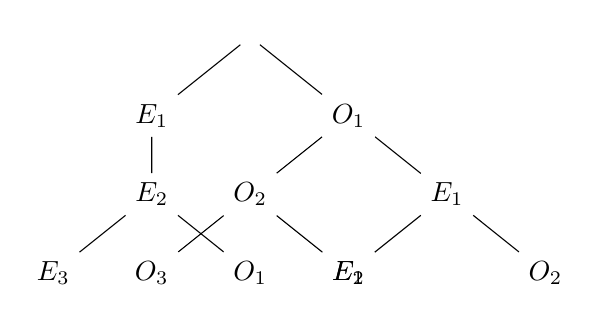
\begin{tikzpicture}[level distance=1.0cm,
nodes={align=center},sibling distance=25mm]

% Nodes
\node{}
	child{node{$E_{1}$} % First Draw Option 1
		child{node{$E_{2}$}
			child{node{$E_{3}$}}
			child{node{$O_{1}$}}
		}
%		child{node{$O_{1}$}
%			child{node{$O_{2}$}}
%			child{node{$E_{2}$}}
%		}
	}
	child{node{$O_{1}$} % First Draw Option 2
		child{node{$O_{2}$}
			child{node{$O_{3}$}}
			child{node{$E_{1}$}}
		}
		child{node{$E_{1}$}
			child{node{$E_{2}$}}
			child{node{$O_{2}$}}
		}
	};

\end{tikzpicture}
			\end{center}
			\begin{enumerate}[label=(\alph*)]
				\item $\Prob \left[ A \Given B \right] = \frac{\Prob \left[ A \cap B \right]}{\Prob \left[ B \right]}$
				\item
			\end{enumerate}
		\end{example}

	\subsection{Event Independence} \label{subsec:Event Independence}
		\begin{definition}[Independent] \label{def:Event Independence}
			Two events $A$ and $B$ are \emph{independent} if
			\begin{equation} \label{eq:Event Independence}
				P \left[ A \cap B \right] = P \left[ A \right] * P \left[ B \right], P\left[ A \right] \neq 0, P\left[ B \right] \neq 0
			\end{equation}
			\begin{itemize}[noitemsep, nolistsep]
				\item If $A \cap B = \emptyset$, the $A$ and $B$ are \textbf{dependent}.
				\item If checking for independence between more than 2 events, you must check each pair, each triple, etc. until you check the independence of each event against each other. For 3 events, $A$, $B$, $C$:
					\begin{itemize}[noitemsep, nolistsep]
						\item Check $P \left[ A \cap B \cap C \right] = P \left[ A \right] * P \left[ B \right] * P \left[ C \right]$
						\item Also need to check:
							\begin{enumerate}[noitemsep, nolistsep]
								\item $P \left[ A \cap B \right] = P \left[ A \right] * P \left[ B \right]$
								\item $P \left[ B \cap C \right] = P \left[ B \right] * P \left[ C \right]$
								\item $P \left[ A \cap C \right] = P \left[ A \right] * P \left[ C \right]$
							\end{enumerate}
					\end{itemize}
			\end{itemize}
		\end{definition}
		\begin{example}[Exam 1, Problem 4]{Event Independence}
			Let $S=\lbrace 1,2,3,4 \rbrace$, and $A = \lbrace 1,2 \rbrace$, $B=\lbrace 1,3 \rbrace$, $C = \lbrace 1,4 \rbrace$, $D = \lbrace 3,4 \rbrace$.
			Assume the outcomes are equiprobable.
			Are the following events independent?
				\begin{enumerate}[noitemsep, nolistsep]
					\item $A$ and $B$
					\item $A$ and $D$
					\item $A$, $B$, and $C$
				\end{enumerate}
		\end{example}
	If 2 events $A$ and $B$ are independent, then their complements are also independent. This is shown in \nameref{proof:Independence of Complements of Events}.
		\begin{proof}[Independence of Complements of Events] \label{proof:Independence of Complements of Events}
			We assumed that $A$ and $B$ were independent, so $P \left[ A \cap B \right] = P \left[ A \right] \cdot P \left[ B \right]$.
			There are 2 more facts we will need:
			\begin{enumerate}[leftmargin=1.0in, label=Fact \arabic*: , ref=Fact \arabic*, noitemsep, nolistsep]
				% leftmargin sets a distance for left margin
				% ref sets the way items will be cross-referenced, and can differ from the label.
				\item $P \left[ B \right] + P \left[ B^{C} \right] = 1$ \label{proof:Independence of Complements of Events:Fact 1}
				\item $P \left[ A \cap B^{C} \right] + P \left[ A \cap B \right] = P \left[ A \right]$ \label{proof:Independence of Complements of Events:Fact 2}
			\end{enumerate}
			From \ref{proof:Independence of Complements of Events:Fact 1}, we have:
			\begin{equation*}
				P \left[ A \cap B \right] = P \left[ A \right] \cdot \left( 1-P \left[ B^{C} \right] \right)
			\end{equation*}
			From \ref{proof:Independence of Complements of Events:Fact 2}, we have $P \left[ A \cap B \right] = P \left[ A \right] - P \left[ A \cap B^{C} \right]$.
			Substituting these into the equation above:
			\begin{align*}
				P \left[ A \right] - P \left[ A \cap B^{C} \right] &= P \left[ A \right] \cdot \left( 1-P \left[ B^{C} \right] \right)\\
				P \left[ A \right] - P \left[ A \cap B^{C} \right] &= P \left[ A \right] - P \left[ A \right] \cdot P \left[ B^{C} \right] \\
				- P \left[ A \cap B^{C} \right] &= -P \left[ A \right] \cdot P \left[ B^{C} \right] \\
				P \left[ A \cap B^{C} \right] &= P \left[ A \right] \cdot P \left[ B^{C} \right] \\
			\end{align*}
			$\therefore$ $A$ and $B^{C}$ are independent, according to the definition of \nameref{def:Event Independence}~events in \Cref{eq:Event Independence}.
		\end{proof}
%%% Local Variables:
%%% mode: latex
%%% TeX-master: "../Math_374-Prob_Stats-Reference_Sheet"
%%% End:
 % Section 3

\section{Counting} \label{sec:Counting}
	\subsection{Sampling \emph{with} Replacement \emph{with} Order} \label{subsec:Ordered Sampling with Replacement}
		\begin{definition} \label{def:Ordered Sampling with Replacement}
			Choose $k$ elements in succession with replacement between selections, from a population of $n$ distinct objects, where $k$ needs to have no relation to $n$.
			\begin{equation} \label{eq:Ordered Sampling with Replacement}
				\frac{n}{First} * \frac{n}{Second} * \frac{n}{Third} * \ldots * \frac{n}{kth \text{ Item}} = n^{k}
			\end{equation}
		\end{definition}
		\begin{example}[Problem 2.42]{Sampling with Replacement with Order}
			A lock has two buttons: a ``0'' button and a ``1'' button.
			To open a door you need to push the buttons according to a preset 8-bit sequence.
			How many sequences are there?
			Suppose you press an arbitrary 8-bit sequence; what is the probability that the door opens? If the first try does not succeed in opening the door, you try another number; what is the probability of success?

			\tcblower

			Solution.
		\end{example}

	\subsection{Sampling \emph{without} Replacement \emph{with} Order} \label{subsec:Ordered Sampling without Replacement}
		\begin{definition} \label{def:Ordered Sampling without Replacement}
			Choose $k$ elements in succession without replacement from a population of $n$ distinct objects, where $k \leq n$
			\begin{equation} \label{eq:Ordered Sampling without Replacement}
				\frac{n}{First} * \frac{n-1}{Second} * \frac{n-2}{Third} * \ldots * \frac{n-k+1}{kth \text{ Item}}
			\end{equation}
		\end{definition}

		\subsubsection{Permutations} \label{subsubsec:Permutations}
			\begin{definition}[Permutation] \label{def:Permutation}
				\emph{Permutations} are special cases of \nameref{subsec:Ordered Sampling without Replacement}, where $k = n$
				\begin{equation} \label{eq:Permutation}
					\frac{n}{First} * \frac{n-1}{Second} * \frac{n-2}{Third} * \ldots * \frac{2}{} * \frac{1}{} * \ldots * \frac{n-k-1}{kth \text{ Item}} = n!
				\end{equation}
			\end{definition}
			\begin{example}[Exam 1, Problem 2]{Password Permutations}
				\begin{enumerate}[noitemsep, nolistsep]
					\item How many unique case-sensitive passswords, of length 8 characters, can be constructed using number (0-9), lower and upper-case letters (a-z, A-Z), and a set of 15 special characters and no spaces?
					\item How many unique passwords if the user must also use at least one integer?
				\end{enumerate}

				\tcblower

				Solution.
			\end{example}

	\subsection{Sampling \emph{with} Replacement \emph{without} Order} \label{subsec:Unordered Sampling with Replacement}
		\begin{definition} \label{def:Unordered Sampling without Replacement}
			Pick $k$ objects from a set of $n$ distinct object with replacement.
			Record the result without order.
			The total number of ways to do this is given in \Cref{eq:Unordered Sampling without Replacement}.
			\begin{equation} \label{eq:Unordered Sampling without Replacement}
				\binom{n+k-1}{k} = \binom{n+k-1}{n-1}
			\end{equation}
		\end{definition}

	\subsection{Sampling \emph{without} Replacement \emph{without} Ordering} \label{subsec:Unordered Sampling without Replacement}
		\begin{definition} \label{def:Unordered Sampling with Replacement}
			Pick $k$ objects from a set of $n$ distinct objects without replacement.
			Record the results with without order.
			We call the resulting subset of $k$ selected objects a ``combination of size $k$.''
			The number of ways to choose $k$ items out of $n$ items is given in \Cref{eq:Unordered Sampling with Replacement}.
			Also said $n$ choose $k$:
			\begin{equation} \label{eq:Unordered Sampling with Replacement}
			\binom{n}{k} = \frac{n * (n-1) * (n-2) * \ldots * (n-k+1)}{k!} = \frac{n!}{k! \left( n-k \right)!}
			\end{equation}
		\end{definition}
		\begin{equation}
			\binom{n}{k} = \binom{n}{n-k}
		\end{equation}
%%% Local Variables:
%%% mode: latex
%%% TeX-master: "../Math_374-Prob_Stats-Reference_Sheet"
%%% End:
 % Section 4

\section{Single Discrete Random Variables}\label{sec:Single Discrete Random Variables}
\begin{definition}[Random Variable]\label{def:Random Variable, Simple}
  A \emph{random variable} $X$ is a function that assigns a real number $X \left( \zeta \right)$ to each outcome $\zeta$ in the sample space of the random experiment.
\end{definition}
\begin{definition}[Discrete Random Variable]\label{def:Discrete Random Variable}
  A \emph{discrete random variable} is a random variable that assumes values in a countable set. For example, the number of heads in 3 coin flips is a discrete random variable.
\end{definition}

\subsection{Probability Mass Function  (PMF)}\label{subsec:Probability Mass Function}
\begin{definition}[Probability Mass Function]\label{def:Probability Mass Function}
  The \emph{probability mass function (PMF)} of a discrete random variable $X$ is defined as:
  \begin{equation}\label{eq:Probability Mass Function}
    p_{X} \left( x \right) = P \left[ X=x \right]
  \end{equation}
  Using the coin example from the definition of a~\nameref{def:Discrete Random Variable},
  \begin{equation}
    p_{X} \left( x \right) =
    \begin{cases}
      \frac{1}{8} & x=0 \\
      \frac{3}{8} & x=1 \\
      \frac{3}{8} & x=2 \\
      \frac{1}{8} & x=3 \\
    \end{cases}
  \end{equation}
\end{definition}
\begin{example}[Problem 3.2]{Probability Mass Function}
  A die is tossed and the random variable $X$ is defined as the number of full pairs of dots on the fact showing up.
  \begin{boldalphlist}[label=\textbf{(\alph*)}, ref=(\alph*)]
  \item Describe the underlying space $S$ of this random experiment and specify the probabilities of the elementary events.\label{ex:3.2a}
  \item Show the mapping from $S$ to $S_{X}$, the range of $S$\label{ex:3.2b}
  \item Find the probabilities for the various values of $X$.\label{ex:3.2c}
  \item Repeat parts \ref{ex:3.2a}, \ref{ex:3.2b}, and \ref{ex:3.2c} if $Y$ is the number of full or partial pairs of dots in the face showing up.
  \item Explain why $\Prob \left[ X = 0 \right]$ and $\Prob \left[ Y = 0 \right]$ are not equal.
  \end{boldalphlist}

  \tcblower

  Solution from Homework 3.
\end{example}

\subsubsection{Properties of Probability Mass Functions}\label{subsubsec:Properties of Probability Mass Functions}
\begin{propertylist}%[label=\textbf{(\roman*)}, noitemsep, nolistsep]
\item
  \begin{equation}
    p_{X} \left( x \right) \geq 0 \text{, } \forall x \in \RealNumbers
  \end{equation}
\item
  \begin{equation}
    \sum\limits_{x \in S_{X}} p_{X} \left( x \right) = 1
  \end{equation}
\end{propertylist}
\begin{example}[Problem 3.13]{Find Normalizing Constant}
  Let $X$ be a random varaible with PMF $p_{k} = \frac{c}{k^{2}}$ for $k = 1,2,\ldots$
  \begin{enumerate}[label=\textbf{(\alph*)}]
  \item Estimate the value of $c$ numerically. Note that the series converges.
  \item Find $\Prob \left[ X > 4 \right]$.
  \item Find $\Prob \left[ 6 \leq X \leq 8 \right]$.
  \end{enumerate}

  \tcblower

  Solution from Homework 4.
\end{example}
\begin{propertylist}[resume]
\item
  \begin{equation}
    P \left[ x \in B \right] = \sum\limits_{x \in B} p_{X} \left( x \right) \text{, where } B \subset S_{X}
  \end{equation}
\end{propertylist}

\subsection{Expected Value/Mean of Single Discrete Random Variable}\label{subsec:Expected Value of Single Discrete}
\begin{definition}[Expected Value/Mean of Single Discrete Random Variable]\label{def:Expected Value of Single Discrete}
  The \emph{expected value} or \emph{mean} of a single discrete random variable $X$ is defined by
  \begin{equation}\label{eq:Expected Value of Single Discrete}
    m_{X} = \ExpectedValue \left[ X \right] = \sum_{x \in S_{X}} x \cdot p_{X} \left( x \right)
  \end{equation}
  \begin{remark}\label{rmk:Expected Value of Single Discrete Countably Infinite}
    If $X$ is countably infinite, you will have an infinite series that exists only if
    \begin{equation}\label{eq:Expected Value of Single Discrete Countably Infinite}
      \sum_{s \in S_{X}} \lvert x \rvert \cdot p_{X} \left( x \right)
    \end{equation}
    is absolutely convergent.
  \end{remark}
\end{definition}
\begin{example}[Problem 3.27]{Expectation of Discrete Random Variable}
  Find the expectation of $X$ where the PMF of $X$ is \[p_{k} = \frac{\frac{pi^{2}}{6}}{k^{2}}\]. (Note that this PMF is the same as in \Cref{ex:Find Normalizing Constant}).

  \tcblower

  Solution from Homework 4. ONLY THE Expectation PART.
\end{example}

\subsubsection{Properties of Expected Values}\label{subsubsec:Properties of Discrete Expected Value}
\begin{definition}[Linearity of Expectation]\label{def:Linearity of Expectation}
  Let $Y = X_{1} + X_{2}$
  \begin{equation}
    \ExpectedValue \left[ X \right] = \ExpectedValue \left[ X_{1} \right] + \ExpectedValue \left[ X_{2} \right]
  \end{equation}
  This can be generalized to
  \begin{equation}\label{eq:General Linearity of Expectation}
    \ExpectedValue \left[ \sum_{i=1}^{k} x_{i} \right] = \sum_{i=1}^{k} \ExpectedValue \left[ X_{i} \right]
  \end{equation}
\end{definition}
\begin{propertylist}
\item
  \begin{equation}
    \ExpectedValue \left[ X_{1} + X_{2} \right] = \ExpectedValue \left[ X_{1} \right] + \ExpectedValue \left[ X_{2} \right]
  \end{equation}
\item
  \begin{equation}
    \ExpectedValue \left[ g \left( X \right) \right] = \sum\limits_{s \in S_{X}} g \left( x \right) \cdot p_{X} \left[ X \right]
  \end{equation}
\item
  \begin{equation}
    \ExpectedValue \left[ c g\left( X \right) \right] = c \ExpectedValue \left[ g\left( X \right) \right]
  \end{equation}
\item
  \begin{equation}
    \ExpectedValue \left[ g_{1} \left( X \right) + g_{2} \left( X \right) + \ldots + g_{m} \left( X \right) \right] = \sum\limits_{i=1}^{m} \ExpectedValue \left[ g_{i} \left( X \right) \right]
  \end{equation}
\end{propertylist}

\subsubsection{Moments of Random Variable}\label{subsubsec:Moments of a Random Variable}
\begin{definition}[Moment]
  The \emph{moment} of a random variable, $X$ is defined as the expectation of the random variable raised to the moment.
  \begin{equation}\label{eq:Moments of a Random Variable}
    \begin{aligned}
      \ExpectedValue \left[ X^{1} \right] &= \text{First Moment} \\
      \ExpectedValue \left[ X^{2} \right] &= \text{Second Moment} \\
      &\vdots \\
      \ExpectedValue \left[ X^{k} \right] &= \text{kth Moment} \\
    \end{aligned}
  \end{equation}
\end{definition}

\subsection{Variance of Single Discrete Random Variable}\label{subsec:Variance of Single Discrete}
\begin{definition}[Variance]\label{def:Variance of Single Discrete}
  The \emph{variance} of a single discrete random variable $X$ is defined as:
  \begin{equation}\label{eq:Variance of Single Discrete-Form 1}
    \ExpectedValue \left[ \left( X - \ExpectedValue \left[ X \right] \right)^{2} \right]
  \end{equation}
  \begin{equation}\label{eq:Variance of Single Discrete-Form 2}
    \Variance \left[ X \right] = \ExpectedValue \left[ X^{2} \right] - \left( \ExpectedValue \left[ X \right] \right)^{2}
  \end{equation}
  and is denoted as $\sigma_{X}^{2}$, or as the operator $\Variance \left[ X \right]$.
  \begin{remark}\label{rmk:Constant in Variance}
    If $X$ is a random variable, and $c$ is some constant coefficient, then:
    \begin{equation}
      \Variance \left[ cX \right] = c^{2} \Variance \left[ X \right]
    \end{equation}
  \end{remark}
\end{definition}
\begin{example}[Problem 3.27]{Variance of Discrete Random Variable}
  Find the variance of $X$ where the PMF of $X$ is \[p_{k} = \frac{\frac{pi^{2}}{6}}{k^{2}}\]. (Note that this PMF is the same as in \Cref{ex:Find Normalizing Constant}).

  \tcblower

  Solution from Homework 4. ONLY THE Variance PART.
\end{example}
\begin{definition}[Standard Deviation]\label{def:Standard Deviation}
  The standard deviation of a random variable $X$ is:
  \begin{equation}\label{eq:Standard Deviation}
    \sigma_{X} = \sqrt{\Variance \left[ X \right]}
  \end{equation}
\end{definition}

\subsection{Conditional Probability Mass Function}\label{subsec:Conditional Probability Mass Function}
\begin{definition}[Conditional Probability Mass of Function]\label{def:Conditional Probability Mass Function}
  Let $X$ be a discrete random variable, with PMF $p_{X} \left( x \right)$ and let $C$ be the event with non-zero probability, i.e. $P \left[ C \right] > 0$.
  The \emph{conditional probability mass function of $X$ given $C$ (Conditional PMF)} is defined as:
  \begin{equation}\label{eq:Conditional Probability Mass Function}
    p_{X \Given C} \left( x \Given C \right) = P \left[ X=x \Given C \right] \text{ for } x \in \RealNumbers
  \end{equation}
  \begin{remark}\label{rmk:Properties of Conditional Probability Mass Functions}
    The conditional PMF, $p_{X \Given C} \left( x \Given C \right)$, satisfies \emph{\textbf{all}} properties of \nameref{subsubsec:Properties of Probability Density Functions}.
  \end{remark}
\end{definition}

\subsection{Conditional Expected Value of Single Discrete Random Variable}\label{subsec:Conditional Expected Value of Single Discrete}
\begin{definition}[Conditional Expected Value of Discrete Random Variable]\label{def:Conditional Expected Value of Single Discrete}
  The \emph{conditional expected value of the discrete random variable} $X$ given $B$ is defined as:
  \begin{equation}\label{eq:Conditional Expected Value of Single Discrete}
    m_{X \Given B} = \ExpectedValue \left[ X \Given B \right] = \sum\limits_{x \in S_{X}} s \cdot p_{X} \left( x \Given B \right)
  \end{equation}
\end{definition}
\begin{example}[Problem 3.39]{Conditional Expected Value}
  \begin{boldalphlist}
  \item Find the conditional expected value of $X$ in Problem 3.5 given that no message gets through in the first time slow. SHow that $\ExpectedValue \left[ X \Given X>1 \right] = \ExpectedValue \left[ X \right] + 1$.\label{ex:3.39a}
  \item Find the conditional expected value of $X$ in problem 3.5 given that a message gets through in the first time slot.\label{ex:3.39b}
  \item Find $\ExpectedValue \left[ X \right]$ by using the results of Parts \ref{ex:3.39a} and \ref{ex:3.39b}.\label{ex:3.39c}
  \item Find $\ExpectedValue \left[ X^{2} \right]$ and $\Variance \left[ X \right]$ using the approach in parts \ref{ex:3.39b} and \ref{ex:3.39c}.
  \end{boldalphlist}

  \tcblower

  Solution from Homework 5.
\end{example}

\subsection{Conditional Variance of Single Discrete Random Variable}\label{subsec:Conditional Variance of Single Discrete}
\begin{definition}[Conditional Variance of Discrete Random Variable]\label{def:Conditional Variance of Single Discrete}
  The \emph{conditional variance of a discrete random variable} $X$ given event $B$ as defined as:
  \begin{equation}\label{eq:Conditional Variance of Single Discrete}
    \begin{aligned}
      \sigma_{X \Given B}^{2} &= \Variance \left[ X \Given B \right] \\
      &= \ExpectedValue \left[ \left( X - \ExpectedValue \left[ X \Given B \right] \right)^{2} \Given B \right] \\
      &= \sum\limits_{x \in S_{X}} \left( x - m_{X \Given B} \right)^{2} \cdot p_{X} \left( x \Given B \right) \\
      \Variance \left[ X \Given B \right] &= \ExpectedValue \left[ X^{2} \Given B \right] - \left( \ExpectedValue \left[ X \Given B \right] \right)^{2} \\
    \end{aligned}
  \end{equation}
\end{definition}
%%% Local Variables:
%%% mode: latex
%%% TeX-master: "../Math_374-Prob_Stats-Reference_Sheet"
%%% End:
 % Section 5

\section{Single Continuous Random Variables}\label{sec:Single Continuous Random Variables}
\begin{definition}[Random Variable]\label{def:Random Variable, Full}
  Consider a random experiment with sample space $S$ and event class $\EventClass$.
  A \emph{random variable} $X$ is a function from the sample space $S$ to the real line $\RealNumbers$ with the property the set $A_{b} = \lbrace \zeta: X \vert \zeta \leq b \rbrace$ is in $\EventClass$ for every $b$ in $\RealNumbers$.
\end{definition}
\begin{definition}[Continuous Random Variable]\label{def:Continuous Random Variable}
  A \emph{continuous random variable} is a random variable whose \nameref{subsec:Cumulative Distribution Function} is continuous everywhere.
\end{definition}

\subsection{Cumulative Distribution Function (CDF)}\label{subsec:Cumulative Distribution Function}
\begin{definition}[Cumulative Distribution Function]\label{def:Cumulative Distribution Function}
  \emph{Cumulative Distribution Function (CDF)} of a random variable $X$ is defined as the probability of the event $\lbrace X \leq x \rbrace$.
  \begin{equation}\label{eq:Cumulative Distribution Function}
    F_{X} \left( x \right) = \Prob \left[ X \leq x \right] \text{ for } -\infty < x < \infty
  \end{equation}
\end{definition}

\subsubsection{Properties of Cumulative Distribution Functions}\label{subsubsec:Properties of Cumulative Distribution Functions}
\begin{propertylist}
\item
  \begin{equation}
    0 \leq F_{X} \left( x \right) \leq 1
  \end{equation}
\item If you include the whole sample space, you should end up with $1$.
  \begin{equation}
    \lim\limits_{x \rightarrow \infty} F_{X} \left( x \right) = 1
  \end{equation}
\item If you exclude the whole sample space, you should end up with $0$.
  \begin{equation}
    \lim\limits_{x \rightarrow -\infty} F_{X} \left( x \right) = 0
  \end{equation}
\item $F_{X} \left( x \right)$ is non-decreasing.
  \begin{equation}
    F_{X} \left( a \right) \leq F_{X} \left( b \right) \text{ if } a \leq b
  \end{equation}
\item The CDF is continuous from the right.
  \begin{equation}
    F_{X} \left( b \right) = \lim\limits_{h \rightarrow 0} F_{X} \left( b+h \right) \text{ where } h>0
  \end{equation}
\item
  \begin{equation}
    \Prob \left[ a<X \leq b \right] = F_{X} \left( b \right) - F_{X} \left( a \right)
  \end{equation}
\item The probability at a point in a CDF. (This usually ends up being $0$).
  \begin{equation}
    \Prob \left[ X=b \right] = F_{X} \left( b \right) - F_{X} \left( b^{-} \right)
  \end{equation}
\item The probability of the event \emph{\textbf{not}} occurring.
  \begin{equation}
    \Prob \left[ X>x \right] = 1 - \Prob \left[ X \leq x \right] =  1 - F_{X} \left( x \right)
  \end{equation}
\end{propertylist}
\begin{example}[Problem 4.29]{Properties of Cumulative Distribution Functions}
  Let $C$ be an event for which $\Prob \left[ C \right] > 0$. Show that $F_{X} \left( X \Given C \right)$ satisfies the 8 properties of a Cumulative Distribution Function.
  \begin{propertylist}
  \item $0 \leq F_{X} \left( x \right) \leq 1$
  \item $\lim \limits_{x \rightarrow \infty} F_{X} \left( x \right) = 1$
  \item $\lim \limits_{x \rightarrow -\infty} F_{X} \left( x \right) = 0$
  \item For $a < b$, $F_{X} \left( a \right) \leq F_{X} \left( b \right)$
  \item $h>0$, $F_{X} \left( b \right) = \lim\limits_{h \rightarrow 0^{+}} F_{X} \left( b+h \right) = F_{X} \left( b^{+} \right)$
  \item $\Prob \left[ a < X \leq b \right] = F_{X} \left( b \right) - F_{X} \left( a \right)$
  \item $\Prob \left[ X = a \right] = F_{X} \left( a \right) - F_{X} \left( a^{-} \right)$
  \item $\Prob \left[ X > x \right] = 1 - F_{X} \left( x \right)$
  \end{propertylist}

  \tcblower

\end{example}

\subsubsection{Conditional Cumulative Distribution Function}\label{subsubsec:Conditional Cumulative Distribution Fuction}
\begin{definition} [Conditional Cumulative Distribution Function]\label{def:Conditional Cumulative Distribution Function}
  The \emph{conditional cumulative distribution function (Conditional CDF)} of $X$ given $C$ is defined by:
  \begin{equation}\label{eq:Conditional Cumulative Distribution Function}
    F_{X \Given C} \left( x \Given C \right) = \frac{P \left[ \lbrace X = x \rbrace \Given C \right]}{\Prob \left[ C \right]}
  \end{equation}
  \begin{remark}
    The conditional CDF, $F_{X \Given C} \left( x \Given C \right)$ satisfies \emph{\textbf{all}} \nameref{subsubsec:Properties of Cumulative Distribution Functions}.
  \end{remark}
\end{definition}
\begin{example}[Problem 4.38]{Conditional Cumulative Distribution Function}
  A binary transmission system sends a ``0'' bit using a -1 voltage signal and a ``1'' by transmitting a +1.
  The received signal is corrupted by noise $N$ that has a Laplacian distribution with parameter $\alpha$.
  Assume that ``0'' and ``1'' bits are equiprobable.
  \begin{boldalphlist}
  \item Find the PDF of the received signal $Y = X+N$ where $X$ is the transmitted signal, given that ``0'' was transmitted; that a ``1'' was transmitted?
  \item Suppose that the receiver decides that a ``0'' was sent if $Y<0$ and a ``1'' was sent if $Y \geq 0$.
    What is the probability that the receiver makes an error given that a +1 was transmitted? A -1 was tramsitted?
  \item What is the overall probability of error?
  \end{boldalphlist}

  \tcblower

  Solution to Problem 4.38 from Homework 7.
\end{example}

\subsection{Probability Density Function (PDF)}\label{subsec:Probability Density Function}
\begin{definition}[Probability Density Function]\label{def:Probability Density Function}
  The \emph{probability density function (PDF)} of a random variable $X$, if it exists, is defined as the derivative of the CDF of $X$.
  \begin{equation}\label{eq:Probability Density Function}
    f_{X} \left( x \right) = \frac{d}{dx} F_{X} \left( x \right)
  \end{equation}
  \begin{remark}\label{rmk:Probability Density Function}
    Both discrete and continuous random variables can have PDFs, however, the discrete random variable will have a discontinuous PDF.
  \end{remark}
  \begin{remark}\label{rmk:Probability Density Function Construction}
    It is possible to construct a random variable that has a \nameref{subsec:Cumulative Distribution Function}, but an undefined \nameref{subsec:Probability Density Function}.
  \end{remark}
  \begin{remark}
    This is an alternate, more useful way to specify the probability law described by the \nameref{subsec:Cumulative Distribution Function}.
  \end{remark}
\end{definition}
\begin{example}[Problem 4.25]{Find Probability Density Function}
  Find the PDF of the Weibull random variable where $\beta = 0.5$, $1$, and $2$.
  \begin{equation*}
    F_{X} \left( x \right) = \begin{cases}
      0 & \text{for } x<0 \\
      1-e^{-\left(\frac{x}{\lambda}\right)^{\beta}} & \text{for } x \geq 0
    \end{cases}
  \end{equation*}

  \tcblower

  Solution to Problem 4.25 from Homework 6.
\end{example}

\subsubsection{Properties of Probability Density Functions}\label{subsubsec:Properties of Probability Density Functions}
These properties apply to PDFs of continuous random variables, and may not hold true for other types of random variables.
\begin{propertylist}
\item The associated CDF is non-decreasing, a \nameref{subsubsec:Properties of Cumulative Distribution Functions}.
  \begin{equation}
    f_{X} \left( x \right) \geq 0
  \end{equation}
\item Since the definition of the PDF is that it's the derivative of the CDF, integrating the space over the PDF will yield the CDF.
  \begin{equation}
    \Prob \left[ a \leq X \leq b \right] = \int_{a}^{b} f_{X} \left( x \right) dx = F_{X} \left( b \right) - F_{X} \left( a \right)
  \end{equation}
\item The value of a location in CDF is the integral of the PDF over the area.
  \begin{equation}
    F_{X} \left( x \right) = \int_{-\infty}^{x} f_{X} \left( t \right) dt
  \end{equation}
\item Including the whole sample space should yield $1$.
  \begin{equation}
    \int_{-\infty}^{\infty} f_{X} \left( x \right) dx = 1
  \end{equation}
\end{propertylist}
\begin{example}[Final Exam Practice Problem 4]{Find Normalizing Constant $c$}
  A random variable $X$ has Probability Distribution Function (PDF):
  \begin{equation*}
    f_{X}\left( x \right) = \begin{cases}
      cx \left( 1- x^{3} \right) & 0 \leq x \leq 1 \\
      0 & \text{otherwise} \\
    \end{cases}
  \end{equation*}
  \begin{enumerate}[noitemsep, nolistsep]
  \item Find the normalizing constant $c$. (5 pts)
  \item Find $P \left[ X = 0.5 \right]$. (3 pts)
  \item Find $P \left[ X > 0.5 \right]$. (7 pts)
  \end{enumerate}

  \tcblower

  Solution to Final Exam Practice Problem 4.
\end{example}
\begin{remark*}
  Any non-negative, piecewise continuous function $g \left( x \right)$ with finite $\int_{-\infty}^{\infty} g \left( x \right) dx = C$ can be used to form a PDF.
\end{remark*}

\subsubsection{Conditional Probability Density Function}\label{subsubsec:Conditional Probability Density Function}
\begin{definition}[Conditional Probability Density Function]\label{def:Conditional Probability Density Function}
  The \emph{conditional probability density function (Conditional PDF)} of $X$ given $C$ is defined by:
  \begin{equation}\label{eq:Conditional Probability Density Function}
    f_{X \Given C} \left( x \Given C \right) = \frac{d}{dx} F_{X \Given C} \left( x \Given C \right)
  \end{equation}
  \begin{remark}
    The conditional PDF, $f_{X \Given C} \left( x \Given C \right)$ satisfies \emph{\textbf{all}} \nameref{subsubsec:Properties of Probability Density Functions}.
  \end{remark}
\end{definition}

\subsection{Expected Value of Single Continuous Random Variable}\label{subsec:Expected Value of Single Continuous}
\begin{definition}[Expected Value/Mean of Random Variable]\label{def:Expected Value of Single Continuous}
  The \emph{expected value of a random variable} $X$, denoted $\ExpectedValue \left[ X \right]$ is defined as:
  \begin{equation}\label{eq:Expected Value of Single Continuous}
    \ExpectedValue \left[ X \right] = \int_{-\infty}^{\infty} t f_{X} \left( t \right) dt
  \end{equation}
  \begin{remark}
    This works with \emph{\textbf{all}} random variables, or general random variables.
  \end{remark}
  \begin{remark}
    $\ExpectedValue \left[ X \right]$ is defined if the integral in \Cref{eq:Expected Value of Single Continuous} converges absolutely.
    This means:
    \begin{equation*}
      \ExpectedValue \left[ X \right] = \int_{-\infty}^{\infty} t f_{X} \left( t \right) dt < \infty
    \end{equation*}
  \end{remark}
\end{definition}
\begin{example}[Problem 4.57]{Conditional Expected Value of Continuous Random Variable}
  Find the $n$th moment of $U$, the uniform random variable in the unit interval.
  Repeat for $X$ uniform in $\left[ a,b \right]$.

  \tcblower

  Solution to Problem 4.57 from Homework 7.
\end{example}

\subsubsection{Properties of Expected Value}\label{subsubsec:Properties of Continuous Expected Value}
\begin{propertylist}
\item The expected value of a function of a random variable.
  \begin{equation}
    \ExpectedValue \left[ h \left( X \right) \right] = \int_{-\infty}^{\infty} h \left( t \right) \cdot f_{X} \left( t \right) dt
  \end{equation}
\item Expectation of a constant, $c$, should be the constant itself.
  \begin{equation}
    \ExpectedValue \left[ c \right] = c
  \end{equation}
\item Sum of a random variable, $X$, and a constant, $c$, is the same as the sum of the expectation of the random variable and the constant.
  \begin{equation}
    \ExpectedValue \left[ X+c \right] = \ExpectedValue \left[ X \right] + \ExpectedValue \left[ c \right]
  \end{equation}
\item Linearity of Expectations for random variables
  \begin{equation}
    \ExpectedValue \left[ a_{0} + a_{1}X + a_{2}X^{2} + \ldots + a_{n}X^{n} \right] = a_{0} + a_{1}\ExpectedValue \left[ X \right] + a_{2}\ExpectedValue \left[ X^{2} \right] + \ldots + a_{n}\ExpectedValue \left[ X^{n} \right]
  \end{equation}
\end{propertylist}

\subsection{Variance of Single Continuous Random Variable}\label{subsec:Variance of Single Continuous}
\begin{definition}[Variance of Random Variable]\label{def:Variance of Single Continuous}
  The \emph{variance} of the random variable $X$ is defined by:
  \begin{equation}\label{eq:Variance of Single Continuous}
    \sigma^{2} = \Variance \left[ X \right] = \ExpectedValue \left[ \left( X - \ExpectedValue \left[ X \right] \right)^{2} \right]
  \end{equation}
  \begin{remark}
    This holds true for \emph{\textbf{all}} types of random variables; discrete, continuous, and mixed.
  \end{remark}
\end{definition}
\begin{definition}[Standard Deviation]\label{def:Standard Deviation of Single Continuous}
  The \emph{standard deviation} of a random variable $X$, denoted by:
  \begin{equation}\label{eq:Standard Deviation of Single Continuous}
    \sigma = \StdDev \left[ X \right] = \sqrt{\Variance \left[ X \right]}
  \end{equation}
  \begin{remark}
    This holds true for \emph{\textbf{all}} types of random variables; discrete, continuous, and mixed.
  \end{remark}
\end{definition}

\subsection{Gaussian/Normal Random Variable}\label{subsec:Gaussian Random Variable}
\begin{definition}[Gaussian/Normal Random Variable]\label{def:Gaussian Random Variable}
  The \emph{Gaussian or normal random variable} is the classic ``bell curve'' probability distribution.
  It is usually described as $X \DrawnFrom N \left( \mu, \sigma^{2} \right)$.
  $\mu$ is $\ExpectedValue \left[ X \right] $ and $\sigma^{2}$ is how narrow/sharp the bell is.
  A Gaussian Random Variable has a PDF of:
  \begin{equation}\label{eq:PDF of Gaussian Random Variable}
    f_{X} \left( x \right) = \frac{1}{\sqrt{2 \pi} \sigma} e^{-\frac{\left( x - \mu \right)^{2}}{2 \sigma^{2}}} \text{, } x \in \RealNumbers
  \end{equation}
\end{definition}
\begin{definition}[Standard Normal Distribution]\label{def:Standard Normal Distribution}
  The \emph{standard normal distribution} is just a specific \nameref{def:Gaussian Random Variable}.
  The standard normal distribution is a \nameref{def:Gaussian Random Variable} with $\mu = 0, \sigma^{2} = 1$.
  \begin{remark}\label{rmk:CDF of Standard Normal Distribution}
    The CDF of the \nameref{def:Standard Normal Distribution} is denoted with $\Phi$.
  \end{remark}
\end{definition}

To find the probability of something for a Gaussian Random Variable, you would end up converting it to the \nameref{def:Standard Normal Distribution}.
If $X \DrawnFrom N \left( \mu, \sigma^{2} \right)$ and $Y \DrawnFrom N \left( 0,1 \right)$,
\begin{equation}\label{eq:Probability of Gaussian Random Variable}
  \begin{aligned}
    \Prob \left[ a \leq x \leq b \right] &= \frac{1}{\sqrt{2 \pi} \sigma} \int_{-\infty}^{\infty} e^{\frac{-1}{2} \left( \frac{x-\mu}{\sigma} \right)^{2}} dx \\
    &= \frac{1}{\sqrt{2 \pi}} \int_{\frac{a-\mu}{\sigma}}^{\frac{b-\mu}{\sigma}} e^{\frac{-1}{2}y}dy \\
    &= P \left[ \frac{a-\mu}{\sigma} \leq Y \leq \frac{b-\mu}{\sigma} \right] \\
    &= F_{Y} \left( \frac{b-\mu}{\sigma} \right) - F_{Y} \left( \frac{a-\mu}{\sigma} \right) \\
    &= \Phi \left( \frac{b-\mu}{\sigma} \right) - \Phi \left( \frac{a-\mu}{\sigma} \right) \\
  \end{aligned}
\end{equation}

\subsubsection{Q-Function}\label{subsubsec:Q-Function}
\begin{definition}[Q-Function]\label{def:Q-Function}
  The \emph{Q-Function} is primarily used in electrical engineering.
  It is defined as:
  \begin{equation}\label{eq:Q-Function}
    \begin{aligned}
      Q &= 1 - \Phi \left( x \right) \\
      &= \frac{1}{\sqrt{2 \pi}} \int_{x}^{\infty} e^{\frac{-t^{2}}{2}} dt \\
    \end{aligned}
  \end{equation}
  \begin{remark}
    \begin{equation}
      Q \left( Z \right) = 1-f_{Z} \left( z \right)
    \end{equation}
  \end{remark}
\end{definition}
\begin{example}[Problem 4.62]{Q-Function Application}
  The $r$th percentile, $\pi \left( r \right)$, of a random variable $X$ is defined by $\Prob \left[ X \leq \pi \left( r \right) \right] = \frac{r}{100}$.
  \begin{boldalphlist}
  \item Find the 90\%, 95\%, and 99\% percentiles of the exponential random variable with parameter $\lambda$.
  \item Repeat part a for the Gaussian random variable with parameters $m=0$ and $\sigma^{2}$.
  \end{boldalphlist}

  \tcblower

  Solution to Problem 4.62 from Homework 7.
\end{example}

\subsection{Markov Inequality}\label{subsec:Markov Inequality}
\begin{definition}[Markov Inequality]\label{def:Markov Inequality}
  Let $X$ be a non-negative random variable with $\ExpectedValue \left[ X \right] < \infty$.
  The \emph{Markov Inequality} states that:
  \begin{equation}\label{eq:Markov Inequality}
    \Prob \left[ X \geq a \right] \leq \frac{\ExpectedValue\left[ X \right]}{a}
  \end{equation}
\end{definition}
\begin{proof}[Proving the Markov Inequality]\label{proof:Markov Inequality}
  \begin{equation*}
    \ExpectedValue \left[ X \right] = \int_{-\infty}^{\infty} x \cdot f_{X} \left( x \right) dx
  \end{equation*}
  Because we defined $X \geq 0$, we change the lower bound to $0$.
  \begin{equation*}
    \ExpectedValue \left[ X \right] = \int_{0}^{\infty} x f_{X} \left( x \right) dx
  \end{equation*}
  We then split the integral up around some point, $a$.
  \begin{equation*}
    \ExpectedValue \left[ X \right] = \int_{0}^{a} x f_{X} \left( x \right) dx + \int_{a}^{\infty} x f_{X} \left( x \right) dx
  \end{equation*}
  Since the first integral is integrating over a non-negative function, the integral is also non-negative.
  \begin{equation*}
    \int_{0}^{a} x f_{X} \left( x \right) dx + \int_{a}^{\infty} x f_{X} \left( x \right) dx \geq \int_{a}^{\infty} x f_{X} \left( x \right) dx
  \end{equation*}
  \begin{equation*}
    \ExpectedValue \left[ X \right] \geq \int_{a}^{\infty} x f_{X} \left( x \right) dx
  \end{equation*}
  Because $x>a$, we can pull a term out of $f_{X} \left( x \right)$
  \begin{equation*}
    \ExpectedValue \left[ X \right] \geq \int_{a}^{\infty} a f_{X} \left(x \right) dx
  \end{equation*}
  Because $a$ is a constant, we pull it out of the integral,
  \begin{equation*}
    \ExpectedValue \left[ X \right] \geq a \int_{a}^{\infty} f_{X} \left( x \right) dx
  \end{equation*}
  Then, we end up with an integral that is the definition of the probability of a continuous random variable.
  \begin{equation*}
    \ExpectedValue \left[ X \right] \geq a \Prob \left[ X \geq a \right]
  \end{equation*}
  \begin{equation*}\label{eq:Proved Markov Inequality}
    \therefore
    \ExpectedValue \left[ X \right] \geq a \Prob \left[ X \geq a \right]
  \end{equation*}
\end{proof}
\begin{example}[Problem 4.97]{Markov Inequality}
  Compare the \nameref{eq:Markov Inequality} and the exact probability for th event $\lbrace X > c \rbrace$ as a function of $c$ for:
  \begin{boldalphlist}
  \item $X$ is a uniform random variable in the interval $\left[ 0,b \right]$.
  \item $X$ is an exponential random variable with parameter $\lambda$.
  \item $X$ is a Pareto random varaible with $\alpha >1$.
  \item $X$ is a Rayleigh random variable.
  \end{boldalphlist}

  \tcblower

  Solution to Problem 4.97 from Homework 7.
\end{example}

\subsection{Chebychev Inequality}\label{subsec:Chebychev Inequality}
\begin{definition}[Chebychev Inequality]\label{def:Chebychev Inequality}
  Let $X$ be a non-negative random variable with $\ExpectedValue \left[ X \right] < \infty$.
  The \emph{Chebychev Inequality} states that:
  \begin{equation}\label{eq:Chebychev Inequality}
    P \left[ \lvert X-\mu \rvert \geq a \right] \leq \frac{\sigma^{2}}{a^{2}}
  \end{equation}
  \begin{proof}[Proving the Chebychev Inequality]\label{proof:Chebychev Inequality}
    \begin{equation*}
      P \left[ \left( X-\mu \right)^{2} \geq a^{2} \right] \leq \frac{\ExpectedValue \left[ \left( X-\mu \right)^{2} \right]}{a^{2}}
    \end{equation*}
    Because $X-\mu = \sigma$, we replace it.
    \begin{equation*}
      P \left[ \left( X-\mu \right)^{2} \geq a^{2} \right] \leq \frac{\ExpectedValue \left[ \sigma^{2} \right]}{a^{2}}
    \end{equation*}
  \end{proof}
\end{definition}
\begin{example}[Problem 4.100]{Chebychev Inequality}
  Let $X$ be the number of successes in $n$ Bernoulli trials were the probability of success is $p$.
  Let $Y = \frac{X}{n}$ be the average number of successes per trial.
  Apply the \nameref{eq:Chebychev Inequality} to the event $\lbrace \lvert Y-p \rvert > a \rbrace$.
  What happens as $n \rightarrow \infty$?

  \tcblower

  Solution to Problem 4.100 from Homework 7.
\end{example}
%%% Local Variables:
%%% mode: latex
%%% TeX-master: "../Math_374-Prob_Stats-Reference_Sheet"
%%% End:
 % Section 6

\section{Multiple Random Variables}\label{sec:Multiple Random Variables}
\subsection[Joint PMF]{Joint Probability Mass Function}\label{subsec:Joint PMF}
\begin{definition}[Joint Probability Mass Function]\label{def:Joint PMF}
  The \emph{joint probability mass function (joint PMF)} of 2 discrete random variables $X$, $Y$ is defined as:
  \begin{equation}\label{eq:Joint PMF}
    p_{X,Y} = P \left[ \lbrace X=x \rbrace \cap \lbrace Y=y \rbrace \right] \text{ for all } x,y \in S_{X,Y}
  \end{equation}
  \begin{itemize}[noitemsep, nolistsep]
  \item This satisfies ALL properties of single random variable PMFs
  \end{itemize}
\end{definition}
\begin{example}[Problem 5.1]{Joint PMF}
  Let $X$ be the maximum and let $Y$ be the minimum of the number of heads obtained when Carlos and Michael each flip a fair coin twice.
  \begin{boldalphlist}
  \item Describe the underlying space $S$ of this random experiment and show the mapping from $S$ to $S_{X,Y}$, the range of the pair $\left( X,Y \right)$.
  \item Find the probability for all values of $\left( X,Y \right)$.
  \end{boldalphlist}

  \tcblower

  Solution to Problem 5.1, Part a \& Part B.
\end{example}

\subsubsection[Marginal PMF]{Marginal Probability Mass Function}\label{subsubsec:Marginal PMF}
\begin{definition}[Marginal Probability Mass Function]\label{def:Marginal PMF}
  Given a joint PMF of discrete random variables $X$, $Y$, the \emph{Marginal Probability Mass Function (Marginal PMF)} of $X$ is defined as:
  \begin{equation}\label{eq:Marginal PMF}
    p_{X} \left( x_{i} \right) = P \left[ X = x_{i} \right] \text{ for } x_{i} \in S_{X}
  \end{equation}
  and is calculated as:
  \begin{equation}\label{eq:Calculate Marginal PMF}
    p \left( x_{i} \right) = \sum_{y \in S_{Y}} p_{X,Y} \left( x_{i}, y \right)
  \end{equation}
\end{definition}
\begin{example}[Problem 5.11]{Marginal PMFs}
  \begin{boldalphlist}
  \item Find the \nameref{def:Marginal PMF}'s for th epairs of random variable with the indicated \nameref{def:Joint PMF}. \\
    \begin{tabular}{cccc|cccc|cccc}
      \hline
      \multicolumn{4}{c|}{i} & \multicolumn{4}{c|}{ii} & \multicolumn{4}{c}{iii} \\ \hline
      $X/Y$ & -1 & 0 & 1 & $X/Y$ & -1 & 0 & 1 & $X/Y$ & -1 & 0 & 1 \\
      -1 & $1/6$ & $1/6$ & 0 & -1 & $1/9$ & $1/9$ & $1/9$ & -1 & $1/3$ & 0 & 0 \\
      0 & 0 & 0 & $1/3$ & 0 & $1/9$ & $1/9$ & $1/9$ & 0 & 0 & $1/3$ & 0 \\
      1 & $1/6$ & $1/6$ & 0 & 1 & $1/9$ & $1/9$ & $1/9$ & 1 & 0 & 0 & $1/3$ \\
      \hline
    \end{tabular} \\ % Extra vertical space here between table and next question

  \item Find the probability of the events $A = \lbrace X>0 \rbrace$, $B = \lbrace X \geq Y \rbrace$, and $C = \lbrace X = -Y \rbrace$ for the above Joint PMF's.
  \end{boldalphlist}

  \tcblower

  Solution to Problem 5.11, Part i \& Part ii \& Part iii.
\end{example}

\subsection[Joint CDF]{Joint Cumulative Distribution Function}\label{subsec:Joint CDF}
\begin{definition}[Joint Cumulative Distribution Function]\label{def:Joint CDF}
  The \emph{Joint Cumulative Distribution Function (Joint CDF)} of $X$ and $Y$ is defined as the probability of the event $ \lbrace X \leq x \rbrace \cap \lbrace Y \leq y \rbrace $
  \begin{equation}\label{eq:Joint CDF}
    \begin{aligned}
      F_{X,Y} \left( x, y \right) &= P \left[ \lbrace X \leq x \rbrace \cap \lbrace Y \leq y \rbrace \right] \text{ for all } \left( x,y \right) \in \mathbb{R}^2 \\
      &= P \left[ \lbrace X \leq x \rbrace , \lbrace Y \leq y \rbrace \right]
    \end{aligned}
  \end{equation}
\end{definition}

\subsubsection{Properties of Joint Cumulative Distribution Functions}\label{subsubsec:Properties of Joint Cumulative Distribution Functions}
\begin{propertylist}
\item $F_{X,Y} \left( x,y \right)$ is non decreasing.
  \begin{equation}\label{eq:Joint CDF Property 1}
    F_{X,Y} \left( x_{1},y_{1} \right) \leq F_{X,Y} \left( x_{2},y_{2} \right) \text{ if } x_{1} \leq x_{2} \text{ and } y_{1} \leq y_{2}
  \end{equation}
\item \begin{equation}\label{eq:Joint CDF Property 2}
    \begin{aligned}
      \lim\limits_{y \rightarrow -\infty} F_{X,Y} \left( x,y \right) &= 0 \\
      \lim\limits_{x \rightarrow -\infty} F_{X,Y} \left( x,y \right) &= 0 \\
      \lim\limits_{\left( x,y \right) \rightarrow \left( \infty, \infty \right)} F_{X,Y} \left( x,y \right) &= 1 \\
    \end{aligned}
  \end{equation}
\item The Marginal CDFs can be obtained from the Joint CDF by removing restrictions for all but one variable.
  \begin{equation}\label{eq:Joint CDF Property 3}
    \begin{aligned}
      F_{X} \left( x \right) &= P \left[ \lbrace X \leq x \rbrace, \lbrace Y \text{ is anything} \rbrace \right] \\
      &= P \left[ \lbrace X \leq x \rbrace, \lbrace -\infty \leq y \leq \infty \rbrace \right] \\
      &= \lim\limits_{y \rightarrow \infty} F_{X,Y} \left( x,y \right) \\
      F_{Y} \left( y \right) &= \lim\limits_{x \rightarrow \infty} F_{X,Y} \left( x,y \right) \\
    \end{aligned}
  \end{equation}
\item The Joint CDF is continuous from $\infty$ to $-\infty$.
  \begin{equation}\label{eq:Joint CDF Property 4}
    \begin{aligned}
      \lim\limits_{x \rightarrow a^{+}} F_{X,Y} \left( x,y \right) &= F_{X,Y} \left( a,y \right) \\
      \lim\limits_{y \rightarrow b^{+}} F_{X,Y} \left( x,y \right) &= F_{X,Y} \left( x,b \right) \\
    \end{aligned}
  \end{equation}
\item The probability of the ``rectangle'' $\lbrace x_{1} \leq X \leq x_{2}, y_{1} \leq Y \leq y_{2} \rbrace$
  \begin{equation}\label{eq:Joint CDF Property 5}
    \begin{aligned}
      P \left[ \lbrace x_{1} \leq X \leq x_{2}, y_{1} \leq Y \leq y_{2} \rbrace \right] &= P \left[ \lbrace X \leq x_{2}, Y \leq y_{2} \rbrace \right] - P \left[ \lbrace X \leq x_{1}, Y \leq y_{2} \rbrace \right] - \\
      &P \left[ \lbrace X \leq x_{2}, Y \leq y_{1} \rbrace \right] + P \left[ \lbrace X \leq x_{1}, Y \leq y_{1} \rbrace \right] \\
      &= F_{X,Y} \left( x_{2}, y_{2} \right) - F_{X,Y} \left( x_{1}, y_{2} \right) - F_{X,Y} \left( x_{2}, y_{1} \right) + F_{X,Y} \left( x_{1}, y_{1} \right)
    \end{aligned}
  \end{equation}
\end{propertylist}

\subsubsection[Marginal CDF]{Marginal Cumulative Distribution Function}\label{subsubsec:Marginal CDF}
\begin{definition}[Marginal Cumulative Distribution Function]\label{def:Marginal CDF}
  We obtain the \emph{Marginal Cumulative Distribution Functions (Marginal CDFs)} by removing the constraint on one of the variables.
  \begin{equation}\label{eq:Marginal CDF}
    \begin{aligned}
      F_{X} \left( x \right) &= P \left[ \lbrace X \leq x \rbrace, \lbrace Y \text{ is anything} \rbrace \right] \\
      &= P \left[ \lbrace X \leq x \rbrace, \lbrace -\infty \leq y \leq \infty \rbrace \right] \\
      &= \lim\limits_{y \rightarrow \infty} F_{X,Y} \left( x,y \right) \\
      F_{Y} \left( y \right) &= \lim\limits_{x \rightarrow \infty} F_{X,Y} \left( x,y \right) \\
    \end{aligned}
  \end{equation}
\end{definition}
\begin{example}[Problem 5.20]{Marginal CDFs}
  The pair $\left( X,Y \right)$ has Joint CDF given by:
  \begin{equation*}
    F_{X,Y} \left( x,y \right) = \begin{cases}
      \left( 1- \frac{1}{x^{2}} \right) \left( 1- \frac{1}{y^{2}} \right) & \text{for } x>1, y>1 \\
      0 & \text{elsewhere}
    \end{cases}
  \end{equation*}
  \begin{boldalphlist}
  \item[\textbf{(b)}] Find the Marginal CDF of $X$ and $Y$.
  \end{boldalphlist}

  \tcblower

  Solution to Problem 5.20, Part b from Homework 8.
\end{example}

\subsection[Joint PDF]{Joint Probability Density Function}\label{subsec:Joint PDF}
\begin{definition}[Joint Probability Density Function]\label{def:Joint PDF}
  We say that $X$, $Y$ are jointly continuous if the probabilities of events involving $X$ and $Y$ can be expressed as an integral of a \emph{Joint Probability Density Function (Joint PDF)}. \newline
  i.e. There exists some non-negative function $f_{X,Y} \left( x,y \right)$, which we call the joint PDF, that is defined on the real plane such that for every event $B$ which is a subset of the xy plane
  \begin{equation}\label{eq:Joint PDF}
    P \left[ \left( X,Y \right) \text{in } B \right] = \iint_{B} f_{X,Y} \left( x,y \right) dx dy
  \end{equation}
  \begin{remark}
    The probability mass of an event is found by integrating the PDF over the region in the xy plane corresponding to your event.
  \end{remark}
\end{definition}


\subsubsection{Properties of Joint Probability Density Functions}\label{subsubsec:Joint PDF Properties}
\begin{propertylist}
\item
  \begin{equation}
    \int_{-\infty}^{\infty} \int_{-\infty}^{\infty} f_{X,Y} \left( x,y \right) = 1
  \end{equation}
\end{propertylist}
\begin{example}[Example 5.16]{Find Normalizing Constant 1}
  Let $X$ be the maximum and $Y$ be the minimum of the number of heads obtained with Carlos and Micahel each flip a fair coin twice.
  Find the Marginal CDF of $X$ and $Y$?

  \tcblower

  Solution to Problem 5.16 from Homework 8.
\end{example}
\begin{example}[Problem 5.27]{Find Normalizing Constant 2}
  Let $X$ and $Y$ have Joint PDF:
  \begin{equation*}
    f_{X,Y} \left( x,y \right) = k x \left( 1-x \right) y \text{, } 0<x<1, 0<y<1
  \end{equation*}
  \begin{boldalphlist}
  \item Find $k$.
  \end{boldalphlist}

  \tcblower

  Solution to Problem 5.27, Part a from Homework 8.
\end{example}
\begin{propertylist}[resume]
\item
  \begin{equation}
    F_{X,Y} \left( x,y \right) = \int_{-\infty}^{x} \int_{-\infty}^{y} f_{X,Y} \left( s,t \right) dt ds
  \end{equation}
\end{propertylist}
\begin{example}[Problem 5.27]{Find Joint CDF}
  Let $X$ and $Y$ have the Joint PDF:
  \begin{equation*}
    f_{X,Y} \left( x,y \right) = k x \left( 1-x \right) y \text{for } 0<x<1, 0<y<1
  \end{equation*}

  \begin{boldalphlist}
  \item Find $k$.
  \item Find the Joint CDF of $\left( X,Y \right)$
  \end{boldalphlist}

  \tcblower

  Solution to Problem 5.27, Part b from Homework 8.
\end{example}
\begin{propertylist}[resume]
\item
  \begin{equation}
    f_{X,Y} = \frac{\partial^{2} f_{X,Y} \left( x,y \right)}{\partial x \partial y}
  \end{equation}
\end{propertylist}

\subsubsection{Marginal PDF}\label{subsubsec:Marginal PDF}
\begin{definition}[Marginal Probability Density Function]\label{def:Marginal PDF}
  The \emph{Marginal Probability Density Functions (Marginal PDFs)} $f_{X} \left( x \right)$ and $f_{Y} \left( y \right)$ are obtained by taking the derivative of the marginal CDFs.
  \begin{equation}
    \begin{aligned}
      f_{X} \left( x \right) &= \frac{d}{dx} F_{X} \left( x \right) \\
      &= \frac{d}{dx} \int_{-\infty}^{x} \left[ \int_{-\infty}^{\infty} f_{X,Y} \left( s,t \right) dt ds \right] \\
      &= \frac{d}{dx} \int_{-\infty}^{x} \int_{-\infty}^{\infty} f_{X,Y} \left( s,t \right) dt ds \\
      &\text{Simplified with \nameref{def:2nd Fundamental Theorem of Calculus}} \\
      &= \int_{-\infty}^{\infty} f_{X,Y} \left( x,t \right) dt \\
      f_{X} &= \int_{-\infty}^{\infty} f_{X,Y} \left( x,t \right) dt \\
    \end{aligned}
  \end{equation}
\end{definition}
\begin{example}[Problem 5.27]{Find Marginal PDFs}
  Let $X$ and $Y$ have the Joint PDF:
  \begin{equation*}
    f_{X,Y} \left( x,y \right) = k x \left( 1-x \right) y \text{for } 0<x<1, 0<y<1
  \end{equation*}
  Find the Marginal DF of $X$ and $Y$?

  \tcblower

  Solution to Problem 5.27, Part c from Homework 8.
\end{example}

\subsection{Independence of Multiple Random Variables}\label{subsec:Independence of Multiple Random Variables}
\begin{definition}[Independent Random Variables]\label{def:Independence of Multiple Random Variables}
  \emph{$X$ and $Y$ are independent random variables} if \emph{\textbf{ANY}} event $A_{1}$ defined in terms of $S$ is independent of \emph{\textbf{ANY}} event $A_{2}$ defined in terms of $Y$.
  \begin{equation}\label{eq:Independence of Multiple Random Variables}
    P \left[ X \in A_{1}, Y \in A_{2} \right] = P \left[ X \in A_{1} \right] * P \left[ Y \in A_{2} \right]
  \end{equation}
\end{definition}
There are 3 ways to phrase this:
\begin{enumerate}[noitemsep, nolistsep]
\item For discrete random variables $X$ and $Y$, $X$ and $Y$ are independent if and only if:
  \begin{equation}\label{eq:Independence of Multiple Discrete Random Variables Using PMF}
    p_{X,Y} \left( x,y \right) = p_{X} \left( x \right) * p_{Y} \left( y \right)
  \end{equation}

\item For general random variables $X$ and $Y$, $X$ and $Y$ are independent if and only if:
  \begin{equation}\label{eq:Independence of Multiple General Random Variables Using CDF}
    F_{X,Y} \left( x,y \right) = F_{X} \left( x \right) * F_{Y} \left( y \right)
  \end{equation}
\end{enumerate}
\begin{example}[Final Exam Practice, Problem 7]{Confirm Independence by PDF}
  Let $X$ and $Y$ have joint Probability Density Function (PDF):
  \begin{equation*}
    f_{X,Y} \left( x,y \right) = \begin{cases}
      12x \left( 1-x \right)y & 0 < x < 1, 0 < y < 1 \\
      0 & \text{otherwise}
    \end{cases}
  \end{equation*}
  Are $X$ and $Y$ independent?
\end{example}
\begin{enumerate}[resume]
\item For (continuous) random variables $X$ and $Y$, $X$ and $Y$ are independent if and only if:
  \begin{equation}\label{eq:Independence of Multiple Continuous Random Variables Using PDF}
    f_{X,Y} \left( x,y \right) = f_{X} \left( x \right) * f_{Y} \left( y \right)
  \end{equation}
\end{enumerate}
\begin{example}[Final Exam Practice, Problem 7]{Confirm Independence by CDF}
  Let $X$ and $Y$ have joint Cumulative Distribution Function (CDF):
  \begin{equation*}
    F_{X,Y} \left( x,y \right) = \begin{cases}
      6y^{2} \left( \frac{x^{2}}{2} - \frac{x^{3}}{3} \right) & 0 < x < 1, 0 < y < 1 \\
      0 & \text{otherwise}
    \end{cases}
  \end{equation*}
  Are $X$ and $Y$ independent?
\end{example}
You can prove \nameref{eq:Independence of Multiple Discrete Random Variables Using PMF}, \Cref{eq:Independence of Multiple Discrete Random Variables Using PMF}.
\begin{proof}[Independence of Discrete Random Variables with PMF]\label{proof:Independence of Discrete Random Variables with PMF}

\end{proof}
\begin{theorem}[Independence of Random Functions]\label{thm:Independence of Random Functions}
  If random variables $X$, $Y$ are independent, then $g\left( X \right)$ and $h \left( Y \right)$ are also independent.
\end{theorem}

\subsection{Expected Value of Functions with 2 Random Variables}\label{subsec:Expected Value of Functions with 2 Random Variables}
\begin{definition}[Expectation of a Function with 2 Random Variables]\label{def:Expectation of a Function with 2 Random Variables}
  Let $Z$ be a random variable described by the function $Z = g \left( X,Y \right)$.
  \begin{equation}\label{eq:Expected Value of a Function with 2 Random Variables}
    \ExpectedValue =
    \begin{cases}
      \int_{-\infty}^{\infty} \int_{-\infty}^{\infty} g \left( x,y \right) \cdot f_{X,Y} \left( x,y \right) dx dy &
      \text{if $X$ and $Y$ are jointly continuous} \\
      \sum\limits_{i \in S_{X}} \sum\limits_{j \in S_{Y}} g \left( x_{i}, y_{j} \right) \cdot p_{X,Y} \left( x,y \right) &
      \text{if $X$ and $Y$ are both discrete} \\
    \end{cases}
  \end{equation}
  \begin{remark}[Expected Value of Sum of Random Variables]\label{rmk:Expected Value of Sum of Random Variables}
    You \emph{\textbf{do not}} need to assume independence to say:
    \begin{equation}\label{eq:Expected Value of Sum of Random Variables}
      \ExpectedValue \left[ X_{1}+X_{2}+\ldots+X_{n} \right] = \ExpectedValue \left[ X_{1} \right] + \ExpectedValue \left[ X_{2} \right] + \ldots + \ExpectedValue \left[ X_{n} \right]
    \end{equation}
  \end{remark}
  \begin{remark}[Expected Value of Product of Random Variables]\label{rmk:Expected Value of Product of Random Variables}
    If $X$ and $Y$ are independent, then
    \begin{equation}\label{eq:Expected Value of Product of Random Variables}
      \ExpectedValue \left[ g \left( X \right) h \left( Y \right) \right] = \ExpectedValue \left[ g \left( X \right) \right] \cdot \ExpectedValue \left[ h \left( Y \right) \right]
    \end{equation}
  \end{remark}
\end{definition}
\begin{example}[Problem 5.56]{Expectation of Multiple Random Variables}
  \begin{boldalphlist}
  \item Find $\ExpectedValue \left[ \left( X+Y \right)^{2} \right]$.
  \item Find $\Variance \left[ X+Y \right]$.
  \item Under what condition is the variance of the sum equal to the sum of the individual variances?
  \end{boldalphlist}

  \tcblower

  Solution to Problem 5.56, Part a from Homework 9.
\end{example}

\subsection{Joint Moments, Correlation, and Covariance}\label{subsec:Joint Moments, Correlation, and Covariance}
\subsubsection{Joint Moments}\label{subsubsec:Joint Moments}
\begin{definition}[The j,kth Moment]\label{def:jkth Moment}
  The \emph{j,kth moment of $X$ and $Y$} is:
  \begin{equation}\label{eq:jkth Moment}
    \ExpectedValue \left[ X^{j} Y^{k} \right] =
    \begin{cases}
      \int_{-\infty}^{\infty} \int_{-\infty}^{\infty} x^{j} y^{k} \cdot f_{X,Y} \left( x,y \right) dx dy &
      \text{if $X$, $Y$ are jointly continuous} \\
      \sum\limits_{i \in S_{X}} \sum\limits_{\ell \in S_{Y}} x_{i}^{j} y_{l}^{k} \cdot p_{X,Y} \left( x_{i},y_{\ell} \right) &
      \text{if $X$, $Y$ are discrete} \\
    \end{cases}
  \end{equation}
\end{definition}

\subsubsection{Correlation}\label{subsubsec:Correlation}
\begin{definition}[Correlation]\label{def:Correlation}
  The \emph{Correlation of $X$ and $Y$} is defined as the $1,1$ moment, i.e. $\ExpectedValue \left[ X^{1} Y^{1} \right]$.
  \begin{remark}
    If $X$, $Y$ are such that $\ExpectedValue \left[ X^{1} Y^{1} \right] = 0$, then we say that $X$, $Y$ are \emph{orthogonal}.
  \end{remark}
  \begin{remark}[Uncorrelated]\label{rmk:Uncorrelated}
    If $X$, $Y$ are such that $\ExpectedValue \left[ XY \right] = \ExpectedValue \left[ X \right] \ExpectedValue \left[ Y \right]$, then $X$ and $Y$ are \emph{uncorrelated}.
  \end{remark}
  \begin{remark}
    If $X$, $Y$ are independent, then they are uncorrelated; but if $X$ and $Y$ are uncorrelated, \emph{\textbf{they are not always independent}}.
  \end{remark}
\end{definition}
\begin{example}[Problem 5.65]{Finding Correlation}
  Let $X$ and $Y$ have Joint PDF:
  \begin{equation*}
    f_{X,Y} \left( x,y \right) = k \left( x+y \right)
  \end{equation*}
  Find the correlation of $X$ and $Y$.
  Determine whether $X$ and $Y$ are independent, orthogonal, or uncorrelated.

  \tcblower

  Solution to Problem 5.65, Everything except Covariance from Homework 9.
\end{example}
\begin{definition}[Correlation Coefficient]\label{def:Correlation Coefficient}
  The \emph{correlation coefficient of $X$, $Y$} is defined as
  \begin{equation}\label{eq:Correlation Coefficient}
    \rho_{X,Y} = \frac{\text{Cov} \left[ X,Y \right]}{\sigma_{X} \sigma_{Y}}
  \end{equation}
  \begin{remark}
    $\rho_{X,Y}$ only ranges $-1 \leq \rho_{X,Y} \leq 1$
  \end{remark}
  \begin{remark}
    The closer $\rho_{X,Y}$ is to $+1$, the closer $X$ and $Y$ are to having a positive linear relationship (Positive slope). \newline
    The closer $\rho_{X,Y}$ is to $-1$, the closer $X$ and $Y$ are to having a negative linear relationship (Negative slope). \newline
    If $\rho_{X,Y} = 0$, the $\text{Cov}\left[ X,Y \right] = 0$, which means that $X$ and $Y$ are \emph{uncorrelated}.
  \end{remark}
\end{definition}

\subsubsection{Covariance}\label{subsubsec:Covariance}
\begin{definition}[Covariance]\label{def:Covariance}
  The \emph{covariance of $X$ and $Y$} is denoted:
  \begin{equation}\label{eq:Covariance-Form 1}
    \text{Cov} \left[ X,Y \right] = \ExpectedValue \left[ \left( X - \ExpectedValue \left[ X \right] \right) \left( Y - \ExpectedValue \left[ Y \right] \right)\right]
  \end{equation}
  \begin{equation}\label{eq:Covariance-Form 2}
    \text{Cov} \left[ X,Y \right] = \ExpectedValue \left[ XY \right] - \ExpectedValue \left[ X \right] \ExpectedValue \left[ Y \right]
  \end{equation}
\end{definition}
\begin{example}[Problem 5.65]{Finding Covariance}
  Let $X$ and $Y$ have Joint PDF:
  \begin{equation*}
    f_{X,Y} \left( x,y \right) = k \left( x+y \right)
  \end{equation*}
  Find the covariance of $X$ and $Y$.
  Using what you found in \Cref{ex:Finding Correlation}, \nameref{ex:Finding Correlation}, determine whether $X$ and $Y$ are independent, orthogonal, or uncorrelated.

  \tcblower
  Solution to Problem 5.65, the Covariance part from Homework 9.
\end{example}

\subsection{Conditional Probability Functions}\label{subsec:Multiple Variable Conditional Probability Functions}
There are 3 major cases for these:
\begin{enumerate}[noitemsep, nolistsep]
\item \nameref{subsubsec:2 Discrete Random Variables}
\item \nameref{subsubsec:1 Discrete 1 Continuous Random Variables}
\item \nameref{subsubsec:2 Continuous Random Variables}
\end{enumerate}

\subsubsection{2 Discrete Random Variables}\label{subsubsec:2 Discrete Random Variables}
\begin{definition}[Conditional Probability Mass Function]\label{def:2 Discrete-Conditional PMF}
  The \emph{conditional Probability Mass Function (Conditional PMF)} of $Y$ given that $X=x$ is:
  \begin{equation}\label{eq:2 Discrete-Conditional PMF}
    p_{Y} \left( y \Given x \right)
    = \frac{P \left[ \lbrace Y=y \rbrace \cap \lbrace X=x \rbrace \right]}{P \left[ X=x \right]}
    = \frac{p_{X,Y} \left( x,y \right)}{p_{X} \left( x \right)}
  \end{equation}
  \begin{remark}
    This also implies that
    \begin{equation}\label{eq:2 Discrete-Joint PMF}
      p_{X,Y} \left( x,y \right) = p_{Y} \left( y \Given x \right) \cdot p_{X} \left( x \right)
    \end{equation}
  \end{remark}
  \begin{remark}
    If $X$ and $Y$ are \emph{independent}, then:
    \begin{equation}\label{eq:2 Discrete-Independent Conditional PMF}
      p_{X} \left( y \Given x \right)
      = \frac{p_{X,Y} \left( x,y \right)}{p_{X} \left( x \right)}
      = \frac{p_{X} \left( x \right) p_{Y} \left( y \right)}{p_{X} \left( x \right)}
      = p_{Y} \left( y \right)
    \end{equation}
  \end{remark}
  \begin{remark}
    The \nameref{def:2 Discrete-Conditional PMF} of 2 discrete random variables satisfies all \nameref{subsubsec:Properties of Probability Mass Functions}.
  \end{remark}
\end{definition}
\begin{example}[Problem 5.75]{Determine Independence of Multiple Discrete Random Variables}
  Need to find new example for this one.
\end{example}

\subsubsection{1 Discrete and 1 Continuous Random Variable}\label{subsubsec:1 Discrete 1 Continuous Random Variables}
For this section, let $X$ be a discrete random variable and $Y$ a continuous random variable.
\begin{definition}[Conditional Cumulative Distribution Function]\label{def:1 Discrete 1 Continuous-Conditional CDF}
  The \emph{conditional Cumulative Distribution Function (Conditional CDF)} of $Y$ given that $X=x$ is:
  \begin{equation}\label{eq:1 Discrete 1 Continuous-Conditional CDF}
    F_{Y} \left( y \Given x \right) = P \left[ Y \leq y \Given X=x \right]
    = \frac{P \left[ \lbrace Y \leq y \rbrace \cap \lbrace X=x \rbrace \right]}{P \left[ X=x \right]}
  \end{equation}
  \begin{remark}
    If $X$ and $Y$ are \emph{independent}, then:
    \begin{equation}\label{eq:1 Discrete 1 Continuous-Independent Conditional CDF}
      F_{Y} \left( y \Given x \right)
      = \frac{F_{X,Y} \left( x,y \right)}{p_{X} \left( x \right)}
      = \frac{F_{Y} \left( y \right) p_{X} \left( x \right)}{p_{X} \left( x \right)}
      = F_{Y} \left( y \right)
    \end{equation}
    This also means that:
    \begin{equation*}
      P \left[ Y \leq y \Given X=x \right]
      = P \left[ Y \leq y \right] \cdot P \left[ X=x \right]
    \end{equation*}
  \end{remark}
  \begin{remark}
    The similar relations for independent random variables with their conditional and marginal probability functions does not hold true with this.
  \end{remark}
  \begin{remark}
    The \nameref{def:1 Discrete 1 Continuous-Conditional CDF} of 1 discrete random variable and 1 continuous random variable satisfies all \nameref{subsubsec:Properties of Cumulative Distribution Functions}.
  \end{remark}
\end{definition}
\begin{definition}[Conditional Probability Density Function]\label{def:1 Discrete 1 Continuous-Conditional PDF}
  The \emph{conditional Probability Distribution Function (Conditional PDF)} of $Y$ given $X=x$ is
  \begin{equation}\label{eq:1 Discrete 1 Continuous-Conditional PDF}
    f_{Y} \left( y \Given x \right) = \frac{d}{dy} F_{Y} \left( y \Given x \right)
  \end{equation}
  This also means,
  \begin{equation*}
    P \left[ Y \leq y \Given X=x \right]
    = \int_{y \in A} f_{Y} \left( y \Given x \right) dy
  \end{equation*}
  \begin{remark}
    The \nameref{def:1 Discrete 1 Continuous-Conditional PDF} of 1 discrete random variable and 1 continuous random variable satisfies all \nameref{subsubsec:Properties of Probability Density Functions}.
  \end{remark}
\end{definition}

\subsubsection{2 Continuous Random Variables}\label{subsubsec:2 Continuous Random Variables}
\begin{definition}[Conditional Cumulative Distribution Function]\label{def:2 Continuous-Conditional CDF}
  The \emph{conditional Cumulative Distribution Function (Conditional CDF)} of $Y$ given $X=x$ for $X$ and $Y$ continuous random variables is:
  \begin{equation}\label{eq:2 Continuous-Conditional CDF}
    F_{Y} \left(y \Given x \right)
    = \lim\limits_{h\rightarrow 0} F_{Y} \left( y \Given x < X \leq \left( x+h \right) \right)
    = \frac{\int_{-\infty}^{y} f_{X,Y} \left( x,v \right) dv}{f_{X} \left( x \right)}
  \end{equation}
  \begin{remark}
    The \nameref{def:2 Continuous-Conditional CDF} of 2 continuous random variables satisfies all \nameref{subsubsec:Properties of Cumulative Distribution Functions}.
  \end{remark}
  \begin{remark}
    The similar relations for the conditional and marginal probability functions do not hold up for 2 continuous random variables too well.
  \end{remark}
\end{definition}

\begin{definition}[Conditional Probability Density Function]\label{def:2 Continuous-Conditional PDF}
  The \emph{conditional Probability Density Function (Conditional PDF)} of $Y$ given $X=x$ for $X$ and $Y$ continuous random variables is:
  \begin{equation}\label{eq:2 Continuous-Conditional PDF}
    f_{Y} \left( y \Given x \right)
    = \frac{d}{dy} F_{Y} \left( y \Given x \right)
    = \frac{f_{X,Y} \left( x,y \right)}{f_{X} \left( x \right)}
  \end{equation}
  \begin{remark}
    If $X$ and $Y$ are independent, then:
    \begin{equation}\label{eq:2 Continuous-Independent Conditional PDF}
      f_{X} \left( y \Given x \right)
      = \frac{f_{X,Y} \left( x,y \right)}{f_{X} \left( x \right)}
      = \frac{f_{X} \left( x \right) f_{Y} \left( y \right)}{f_{X} \left( x \right)}
      = f_{Y} \left( y \right)
    \end{equation}
  \end{remark}
  \begin{remark}
    The \nameref{def:2 Continuous-Conditional PDF} of 2 continuous random variables satisfies all \nameref{subsubsec:Properties of Probability Density Functions}.
  \end{remark}
\end{definition}

\subsection{Conditional Expectation of Multiple Random Variables}\label{subsec:Conditional Expectation of Multiple Variables}
\begin{definition}[Conditional Expectation]\label{def:Conditional Expectation of Multiple Variables}
  The \emph{conditional expectation} of $Y$ given $X$ is:
  \begin{equation}\label{eq:Conditional Expectation of Multiple Variables}
    \ExpectedValue \left[ Y \Given X=x \right] = \int_{-\infty}^{\infty} y \cdot f_{Y} \left( y \Given x \right) dy
  \end{equation}
  \begin{remark}[Special Case]
    There is a special case when \emph{\textbf{both}} $X$ and $Y$ are discrete random variables.
    \begin{equation}\label{eq:Conditional Expectation of Multiple Discrete Variables}
      \ExpectedValue \left[ Y \Given X=x \right] = \sum_{y \in S_{Y}} y \cdot p_{Y} \left( y \Given x \right)
    \end{equation}
  \end{remark}
  \begin{remark}
    When calculating the \nameref{subsec:Conditional Expectation of Multiple Variables}, and they as for $\ExpectedValue \left[ Y \Given X=x \right]$, that means you \emph{\textbf{must}} consider all possible values that $X$ can take.
    This can be generalized to the equation below.
    \begin{equation}\label{eq:General Conditional Expectation of Multiple Variables}
      \ExpectedValue \left[ Y \Given X=x \right] = \sum_{x \in S_{X}} \left( \sum_{y \in S_{Y}} y \cdot p_{Y} \left( y \Given x \right) \right)
    \end{equation}
    This can be described. You must take a single value for $x$, and take it over all $y$'s, then take the next value for $x$, until you have exhausted all values in both $S_{X}$ and $X_{Y}$. \newline
    This can also be translated into the continuous case, but the discrete case is a little simpler to understand this generality.
  \end{remark}
  \begin{remark}
    $\ExpectedValue \left[ Y \Given X=x \right]$ is a function of $X$, so it can be written as $g \left( x \right) = \ExpectedValue \left[ Y \Given X=x \right]$.
    Thus, we can also say
    \begin{equation}\label{eq:Expected Value of Conditional Expected Value of Multiple Variables}
      \ExpectedValue \left[ g \left( x \right) \right] = \ExpectedValue \left[ \ExpectedValue \left[ Y \Given X \right] \right] = \ExpectedValue \left[ Y \right]
    \end{equation}
    \begin{subequations}
      \begin{align}\label{eq:Joint PDF of Multiple Continuous Random Variables}
        \ExpectedValue \left[ Y \right]
        = \ExpectedValue \left[ \ExpectedValue \left[ Y \Given X \right] \right]
        &= \int_{-\infty}^{\infty} \ExpectedValue \left[ Y \Given x \right] f_{X} \left( x \right) dx
          = \int_{-\infty}^{\infty} \int_{-\infty}^{\infty} y f_{Y} \left( y \Given x \right) dy f_{X} \left( x \right) dx \\
       \label{eq:Joint PDF of Multiple Discrete Random Variables}
        \ExpectedValue \left[ Y \right]
        = \ExpectedValue \left[ \ExpectedValue \left[ Y \Given X \right] \right]
        &= \sum_{x \in S_{X}} \ExpectedValue \left[ Y \Given x \right] p_{X} \left( x \right)
          = \sum_{x_{j} \in S_{X}} \sum_{y_{i} \in S_{Y}} y_{i} p_{Y} \left( y_{i} \Given x_{k} \right) p_{X} \left( x_{j} \right)
      \end{align}
    \end{subequations}
  \end{remark}
\end{definition}
\begin{proof}[Prove Expectation of Conditional Expected Value]\label{proof:Expected Value of Conditional Expected Value of Multiple Variables}
\end{proof}
\begin{example}[Problem 5.75]{Finding Conditional Expected Value}
  Let $X$ be the maximum and let $Y$ be the minimum of the number of heads obtained when Carlos and Michael each flip a coin twice.
  \begin{boldalphlist}
  \item Find $p_{Y} \left( y \Given x \right)$ and $p_{x} \left( x \Given y \right)$, assuming fair coins are used.\label{prob:5.75a}
  \item Find $p_{Y} \left( y \Given x \right)$ and $p_{x} \left( x \Given y \right)$, assuming Carlos uses a coin with $p = \frac{3}{4}$.\label{prob:5.75b}
  \item Find $\ExpectedValue \left[ Y \Given X=x \right]$ and $\ExpectedValue \left[ X \Given Y=y \right]$ in part \ref{prob:5.75a}; then find $\ExpectedValue \left[ X \right]$ and $\ExpectedValue \left[ Y \right]$.
  \item Find $\ExpectedValue \left[ Y \Given X=x \right]$ and $\ExpectedValue \left[ X \Given Y=y \right]$ in part \ref{prob:5.75b}; then find $\ExpectedValue \left[ X \right]$ and $\ExpectedValue \left[ Y \right]$.
  \end{boldalphlist}

  \tcblower

  Solution to Problem 5.75, Part e from Homework 10.
\end{example}
%%% Local Variables:
%%% mode: latex
%%% TeX-master: "../Math_374-Prob_Stats-Reference_Sheet"
%%% End:
 % Section 7

\section{Random Vectors}\label{sec:Random Vectors}
Random Vectors are usually denoted:
\begin{equation}\label{eq:Random Vector Notation}
  \vec{X} = \langle X_{1}, X_{2} X_{3}, \ldots, X_{n} \rangle
\end{equation}
\begin{definition}[Random Vector]\label{def:Random Vector}
  A \emph{random vector} is a list of \nameref{def:Random Variable, Full}s.
  \begin{remark}
    Almost all of the material for \nameref{sec:Multiple Random Variables} is applicable here.
    However, the 2 random variable equations and definitions must be generalized to $n$ random variables.
  \end{remark}
\end{definition}

\subsection{Joint CDF of a Random Vector}\label{subsec:Joint CDF of Random Vector}
This is just the generalization of \nameref{def:Joint CDF} to $n$ random variables.
\begin{equation}\label{eq:Joint CDF of Random Vector}
  \begin{aligned}
    F_{\vec{X}} \left( \vec{x} \right)
    &= F_{X_{1}, X_{2}, X_{3}, \ldots, X_{n}} \left( x_{1}, x_{2}, x_{3}, \ldots, x_{n} \right) \\
    &= P \left[ X_{1} \leq x_{1}, X_{2} \leq x_{2}, X_{3} \leq x_{3}, \ldots, X_{n} \leq x_{n} \right] \\
  \end{aligned}
\end{equation}

\subsection{Joint PDF of a Random Vector}\label{subsec:Joint PDF of Random Vector}
This is just the generalization of \nameref{def:Joint PDF} to $n$ random variables.
\begin{equation}\label{eq:Joint PDF of Random Vector}
  f_{\vec{X}} \left( \vec{x} \right) = \frac{\partial^{n} F_{\vec{X}} \left( \vec{x} \right)}{\partial x_{1} \partial x_{2} \partial x_{3} \cdots \partial x_{n}}
\end{equation}

\subsubsection{Marginal PDF of a Random Vector}\label{subsubsec:Marginal PDF of Random Vector}
This is just the generalization of \nameref{def:Marginal PDF} to $n$ random variables.
Integrate out the terms that you're not interested in.
\begin{equation}\label{eq:Marginal PDF of Random Vector}
  f_{\vec{X}} = \int_{-\infty}^{\infty} \cdots \int_{-\infty}^{\infty} f_{\vec{X}} \left( \vec{x} \right) \partial x_{2} \partial x_{3} \cdots \partial x_{n}
\end{equation}
For instance, say we want the marginal PDF of some function with respect to $X_{1}$, $X_{3}$, and $X_{4}$.
\begin{equation}\label{eq:Marginal PDF of Random Vector Multiple Variables}
  f_{X_{1}, X_{3}, X_{4}} \left( x_{1}, x_{3}, x_{4} \right) = \int_{-\infty}^{\infty} \cdots \int_{-\infty}^{\infty} f_{\vec{X}} \left( \vec{x} \right) \partial x_{2} \partial x_{5} \partial x_{6} \cdots \partial x_{n}
\end{equation}

\subsection{Conditional Probability Functions of Random Vectors}\label{subsec:Random Vector Conditional Probability Functions}
This section is just an extension of \Cref{subsec:Multiple Variable Conditional Probability Functions}, \nameref{subsec:Multiple Variable Conditional Probability Functions}.
There are 3 major cases for these:
\begin{enumerate}[noitemsep, nolistsep]
\item \nameref{subsubsec:Conditional Probability Discrete Random Vectors}
\item \nameref{subsubsec:Conditional Probability Mixed Random Vectors}
\item \nameref{subsubsec:Conditional Probability Continuous Random Vectors}
\end{enumerate}

\begin{remark*}\label{rmk:Define Random Vector Y for Example}
  \begin{large}
    For the sections below, let $\vec{Y}= \langle Y_{1},Y_{2},Y_{3} \rangle$ and $\vec{y}= \langle y_{1},y_{2},y_{3} \rangle$.
  \end{large} \newline
  While I am using $\vec{Y}$ and $\vec{y}$, these equations can be further generalized to higher dimensions.
  All that would be required for this is to keep track of everything.
\end{remark*}

\subsubsection{Discrete Random Vectors}\label{subsubsec:Conditional Probability Discrete Random Vectors}
\begin{definition}[Discrete Random Vector Conditional Probability Mass Function]\label{def:Discrete Random Vector-Conditional PMF}
  The \emph{conditional Probability Mass Function (Conditional PMF)} of $Y_{3}$ given that $Y=y$ is:
  \begin{equation}\label{eq:Discrete Random Vector-Conditional PMF}
    p_{Y_{3}} \left( y_{3} \Given y_{1},y_{2} \right)
    = \frac{P \left[ \lbrace Y_{3}=y_{3} \rbrace \cap \left( \lbrace Y_{1}=y_{1} \rbrace \cap \lbrace Y_{2}=y_{2} \rbrace \right) \right]}{P \left[ \lbrace Y_{1}=y_{1} \rbrace \cap \lbrace Y_{2}=y_{2} \rbrace \right]}
    = \frac{p_{\vec{Y}} \left( \vec{y} \right)}{p_{Y_{1},Y_{2}} \left( y_{1},y_{2} \right)}
  \end{equation}
  \begin{remark}
    This also implies that
    \begin{equation}\label{eq:Discrete Random Vector-Joint PMF}
      p_{\vec{Y}} \left( \vec{y} \right) = p_{Y_{3}} \left( y_{3} \Given y_{1},y_{2} \right) \cdot p_{Y_{2}} \left( y_{2} \Given y_{1} \right) \cdot p_{Y_{1}} \left( y_{1} \right)
    \end{equation}
  \end{remark}
  \begin{example}[Problem 6.11]{Conditional PMFs Yield Joint PMF}
    Show that $f_{X,Y,Z} \left( x,y,z \right) = f_{Z} \left( z \Given x,y \right) f_{Y} \left( y \Given x \right) f_{X} \left( x \right)$.

    \tcblower

    Solution to Problem 6.11 from Homework 10.
  \end{example}
  \begin{remark}
    If all elements of $\vec{Y}$ are \emph{independent} (Remember that you need to check each subgroup too, like shown in \Cref{subsec:Event Independence}), then:
    \begin{equation}\label{eq:Discrete Random Vector-Independent Conditional PMF}
      p_{Y_{3}} \left( y_{3} \Given y_{1},y_{2} \right)
      = \frac{p_{\vec{Y}} \left( \vec{y} \right)}{p_{Y_{1},Y_{2}} \left( y_{1},y_{2} \right)}
      = \frac{p_{Y_{1},Y_{2}} \left( y_{1},y_{2} \right) p_{Y_{3}} \left( y_{3} \right)}{p_{Y_{1},Y_{2}} \left( y_{1},y_{2} \right)}
      = p_{Y_{3}} \left( y_{3} \right)
    \end{equation}
  \end{remark}
  \begin{remark}
    The \nameref{def:Discrete Random Vector-Conditional PMF} of 2 discrete random variables satisfies all \nameref{subsubsec:Properties of Probability Mass Functions}.
  \end{remark}
\end{definition}

\subsubsection{Mixed Random Vectors}\label{subsubsec:Conditional Probability Mixed Random Vectors}
Because of the continuous random variable present in the random vector, we can describe a mixed random vector with either:
\begin{enumerate}[noitemsep, nolistsep]
\item \nameref{def:Mixed Random Vector-Conditional CDF}
\item \nameref{def:Mixed Random Vector-Conditional PDF}
\end{enumerate}
\begin{definition}[Mixed Random Vector Conditional CDF]\label{def:Mixed Random Vector-Conditional CDF}
  The \emph{conditional Cumulative Distribution Function (CDF)} of $Y$ given that $X = x$ is:
  \begin{equation}\label{eq:Mixed Random Vector-Conditional CDF}
    F_{Y} \left( y \Given x \right) = \Prob \left[ Y \leq y \Given X=x \right] = \frac{\Prob \left[ \lbrace Y \leq y \rbrace \cap \lbrace X = x \rbrace \right]}{\Prob \left[ X = x \right]} \text{for } \Prob \left[ X = x \right] >0
  \end{equation}
  \begin{remark}
    If $X$ and $Y$ are independent, then:
    \begin{equation}\label{eq: Mixed Random Vector-Independent-Conditional CDF}
      \begin{aligned}
        \Prob \left[ Y \leq y \Given X=x \right] &= \Prob \left[ Y \leq y \right] \cdot \Prob \left[ X = x \right] \\
        &= F_{Y} \left( y \right) \cdot p_{X} \left( x \right)
      \end{aligned}
    \end{equation}
  \end{remark}
  \begin{remark}
    The \nameref{def:Mixed Random Vector-Conditional CDF} of mixed random variables satisfies all \nameref{subsubsec:Properties of Cumulative Distribution Functions}.
  \end{remark}
\end{definition}
\begin{definition}[Mixed Random Vector Conditional PDF]\label{def:Mixed Random Vector-Conditional PDF}
  The \emph{conditional Probability Density Function (PDF)} of $Y$ given that $X=x$ is:
  \begin{equation}\label{eq:Mixed Random Vector-Conditional PDF}
    f_{Y} \left( y \Given x \right) = \frac{d}{dy} F_{Y} \left( y \Given x \right)
  \end{equation}
  \begin{remark}
    In this case, we only take the derivative with respect to the continuous random variable because the discrete random variables are constant.
  \end{remark}
  \begin{remark}
    The \nameref{def:Mixed Random Vector-Conditional PDF} of mixed random variables satisfies all \nameref{subsubsec:Properties of Probability Density Functions}.
  \end{remark}
\end{definition}

\subsubsection{Continuous Random Vectors}\label{subsubsec:Conditional Probability Continuous Random Vectors}
\begin{definition}[Continuous Random Vector Conditional CDF]\label{def:Continuous Random Vector-Conditional CDF}
  The \emph{conditional Cumulative Distribution Function (CDF)} of a continuous random vector of $Y$ given $X=x$, where both $Y$ and $X$ are continuous random variables is given below.
  \begin{equation}
    \begin{aligned}
      F_{Y} \left( y \Given x \right) &= \lim\limits_{h \rightarrow 0} F_{Y} \left( y \Given x < X \leq x+h \right) \\
      &= \frac{\int_{-\infty}^{y} f_{X,Y} \left( x,v \right) dv}{f_{X} \left( x \right)} \\
    \end{aligned}
  \end{equation}
  \begin{remark}
    Since $X$ is a continuous random variable, $\Prob \left[ X=x \right] =0$.
    So, we must use limits to get an infinitely close approximation, so: $\lim \limits_{h \rightarrow 0} \Prob \left[ x < X \leq x+h \right]$.
  \end{remark}
  \begin{remark}
    The \nameref{def:Continuous Random Vector-Conditional CDF} satisfies all \nameref{subsubsec:Properties of Cumulative Distribution Functions}.
  \end{remark}
\end{definition}
\begin{definition}[Continuous Random Vector Conditional PDF]\label{def:Continuous Random Vector-Conditional PDF}
  The \emph{conditional Probability Density Function (PDF)} of a continuous random vector of $Y$ given $X=x$, where both $Y$ and $X$ are continuous random variables is given below.
  \begin{equation}
    \begin{aligned}
      f_{Y} \left( y \Given x \right) &= \frac{d}{dy} F_{Y} \left( y \Given x \right) \\
      &= \frac{f_{X,Y} \left( x,y \right)}{f_{X} \left( x \right)} \\
    \end{aligned}
  \end{equation}
  \begin{remark}
    This can be done both ways:
    \begin{enumerate}[noitemsep, nolistsep]
    \item \begin{equation*}
        f_{X,Y} \left( x,y \right) = f_{Y} \left( y \Given x \right) \cdot f_{X} \left( x \right)
      \end{equation*}
    \item \begin{equation*}
        f_{X,Y} \left( x,y \right) = f_{X} \left( x \Given y \right) \cdot f_{X} \left( y \right)
      \end{equation*}
    \end{enumerate}
  \end{remark}
  \begin{remark}
    The \nameref{def:Continuous Random Vector-Conditional PDF} satisfies all \nameref{subsubsec:Properties of Probability Density Functions}.
  \end{remark}
\end{definition}
\begin{example}[Example 5.32]{Find Conditional PDF of Continuous Random Vector}
  Let $X$ and $Y$ be jointly continuous random variables.
  \begin{equation*}
    \begin{aligned}
      f_{X,Y} \left( x,y \right) &= \begin{cases}
        2 e^{-x} e^{-y} & 0 \leq x \leq y \leq \infty \\
        0 & \text{otherwise}
      \end{cases}
      f_{X} \left( x \right) &= 2 e^{-x} \left( 1-e^{-x} \right) \text{for } 0 \leq x \leq \infty \\
      f_{Y} \left( y \right) &= 2 e^{-y} \text{for } 0 \leq y \leq \infty \\
    \end{aligned}
  \end{equation*}
  \begin{enumerate}[noitemsep, nolistsep]
  \item Find $f_{X} \left( x \Given y \right)$.
  \item Find $f_{Y} \left( y \Given x \right)$.
  \end{enumerate}

  \tcblower

  Solution to Example 5.32 from Lecture 23.
\end{example}

\subsection{Mean Vector}\label{subsec:Mean Vector}
\begin{definition}[Mean Vector]\label{def:Mean Vector}
  For $\vec{X} = \langle X_{1},X_{2},\ldots,X_{n} \rangle$, the \emph{mean vector} is defined as the column vector of expected values of the components of $X_{k}$:
  \begin{equation}\label{eq:Mean Vector}
    \mathbf{m_{X}}
    = \ExpectedValue \left[ \vec{X} \right]
    = \begin{bmatrix}
      X_{1} \\
      X_{2} \\
      \vdots \\
      X_{n}
    \end{bmatrix}
    \triangleq \begin{bmatrix}
      \ExpectedValue \left[ X_{1} \right] \\
      \ExpectedValue \left[ X_{2} \right] \\
      \vdots \\
      \ExpectedValue \left[ X_{n} \right] \\
    \end{bmatrix}
  \end{equation}
  \begin{remark}
    Note that we defined the vector of expected values as a column vector.
    Other texts will use row vectors for other things, but the use of column vectors here is intentional.
  \end{remark}
\end{definition}
\begin{example}[Problem 6.35]{Finding Mean Vector}
  Let $X, Y, Z$ have joint PDF
  \begin{equation*}
    f_{X,Y,Z} \left( x,y,z \right) = \frac{2}{3} \left( x+y+z \right) \text{for } 0 \leq x \leq 1, 0 \leq y \leq 1, 0 \leq z \leq 1
  \end{equation*}
  Find the mean vector for $\left( X,Y,Z \right)$.

  \tcblower

  Solution to Problem 6.35, ONLY Mean Vector Part, from Homework 10.
\end{example}

\subsection{Correlation and Covariance Matrix}\label{subsec:Correlation and Correlation Matrix}
\begin{definition}[Correlation Matrix]
  The \emph{correlation matrix} has the second moments of $\bar{X}$ as its entries:
  \begin{equation}\label{eq:Correlation Matrix}
    \mathbf{\bar{R}_{X}}
    = \begin{bmatrix}
      \ExpectedValue \left[ X_{1}^{2} \right] & \ExpectedValue \left[ X_{1}X_{2} \right] & \cdots & \ExpectedValue \left[ X_{1}X_{n} \right] \\
      \ExpectedValue \left[ X_{2}X_{1} \right] & \ExpectedValue \left[ X_{2}^{2} \right] & \cdots & \ExpectedValue \left[ X_{2}X_{n} \right] \\
      \vdots & \vdots & \ddots & \vdots \\
      \ExpectedValue \left[ X_{n}X_{1} \right] & \ExpectedValue \left[ X_{n}X_{2} \right] & \cdots & \ExpectedValue \left[ X_{n}^{2} \right] \\
    \end{bmatrix} \\
  \end{equation}
  \begin{remark}
    $\bar{R}_{X}$ is a $n \times n$ symmetric matrix.
  \end{remark}
\end{definition}
\begin{definition}[Covariance Matrix]\label{def:Covariance Matrix}
  The \emph{covariance matrix} has the second-order central moments as its entries:
  \begin{equation}\label{eq:Covariance Matrix}
    \begin{aligned}
      \mathbf{\bar{K}_{X}}
      &= \begin{bmatrix}
        \ExpectedValue \left[ \left( X_{1} - m_{1} \right)^{2} \right] & \ExpectedValue \left[ \left( X_{1}-m_{1} \right) \left( X_{2}-m_{2} \right) \right] & \cdots & \ExpectedValue \left[ \left( X_{1}-m_{1} \right) \left( X_{n}-m_{n} \right) \right] \\
        \ExpectedValue \left[ \left( X_{2}-m_{2} \right) \left( X_{1}-m_{1} \right) \right] & \ExpectedValue \left[ \left( X_{2}-m_{2} \right)^{2} \right] & \cdots & \ExpectedValue \left[ \left( X_{2}-m_{2} \right) \left( X_{n}-m_{n} \right) \right] \\
        \vdots & \vdots & \ddots & \vdots \\
        \ExpectedValue \left[ \left( X_{n}-m_{n} \right) \left( X_{1}-m_{1} \right) \right] & \ExpectedValue \left[ \left( X_{n}-m_{n} \right) \left( X_{2}-m_{2} \right) \right] & \cdots & \ExpectedValue \left[ \left( X_{n}-m_{n} \right)^{2} \right] \\
      \end{bmatrix} \\
      &= \begin{bmatrix}
        \Variance \left[ X_{1} \right] & \Covariance \left[X_{1},X_{2} \right] & \cdots & \Covariance \left[ X_{1},X_{n} \right] \\
        \Covariance \left[ X_{2},X_{1} \right] & \Variance \left[ X_{2} \right]  & \cdots & \Covariance \left[ X_{2},X_{n} \right] \\
        \cdots & \cdots & \ddots & \cdots \\
        \Covariance \left[ X_{n},X_{1} \right] & \Covariance \left[ X_{2},X_{n} \right] & \cdots & \Variance \left[ X_{n} \right] \\
      \end{bmatrix}
    \end{aligned}
  \end{equation}
  \begin{remark}
    $\bar{K}_{X}$ is a $n \times n$ symmetric matrix.
  \end{remark}
  \begin{remark}
    The diagonal elements of $\bar{K}_{X}$ are given by the variances $\Variance \left[ X_{k} \right] = \ExpectedValue \left[ \left( X_{k}-m_{k} \right)^{2} \right]$ of the elements of $\vec{X}$.
  \end{remark}
  \begin{remark}
    If the diagonal elements of $\bar{K}_{X}$ are \nameref{rmk:Uncorrelated}, then $\Covariance \left[ X_{j}, X_{k} \right] = 0$ for $j \neq k$, and $\bar{K}_{X}$, the \nameref{def:Covariance Matrix} is a diagonal matrix.
  \end{remark}
  \begin{remark}
    If the random variables $X_{1},X_{2},\cdots,X_{n}$ are independent, then they are uncorrelated and $\bar{K}_{X}$ is diagonal.
  \end{remark}
  \begin{remark}
    If the \nameref{def:Mean Vector} is $\bar{0}$, that is, $m_{k} = \ExpectedValue \left[ X_{k} \right] = 0$ for all $k$, then $\bar{R}_{X} = \bar{K}_{X}$.
  \end{remark}
\end{definition}
\begin{example}[Problem 6.35]{Find Covariance Matrix}
  Let $X, Y, Z$ have joint PDF
  \begin{equation*}
    f_{X,Y,Z} \left( x,y,z \right) = \frac{2}{3} \left( x+y+z \right) \text{for } 0 \leq x \leq 1, 0 \leq y \leq 1, 0 \leq z \leq 1
  \end{equation*}
  Find the covariance matrix for $\left( X,Y,Z \right)$.

  \tcblower

  Solution to Problem 6.35, Only Covariance Matrix part, from Homework 10.
\end{example}
%%% Local Variables:
%%% mode: latex
%%% TeX-master: "../Math_374-Prob_Stats-Reference_Sheet"
%%% End:
 % Section 8

\section{Sums of Random Variables}\label{sec:Sums of Random Variables}
\begin{definition}[Sum of Random Variables]\label{def:Sum of Random Variables}
  The definition of a \emph{sum of random variables} is given in \Cref{eq:Sum of Random Variables} below.
  Where $X_{i}$ is a random variable,
  \begin{equation}\label{eq:Sum of Random Variables}
    S_{n} = \sum_{i=1}^{n} X_{i} = X_{1} + X_{2} + \ldots + X_{n}
  \end{equation}
\end{definition}

\subsection{Means and Variances of Sums of Random Variables}\label{subsec:Means and Variances of Sums of Random Variables}
\begin{definition}[Mean of Sums of Random Variables]\label{def:Mean of Sums of Random Variables}
  The \emph{mean of sums of random variables} is the same as the \emph{expected value of sums of random variables}.
  \begin{equation}
    \ExpectedValue \left[ S_{n} \right] = \sum_{i=1}^{n} \ExpectedValue \left[ X_{i} \right]
  \end{equation}
  \begin{remark}
    All the properties of \nameref{subsubsec:Properties of Discrete Expected Value} and/or \nameref{subsubsec:Properties of Continuous Expected Value} hold true here as well..
  \end{remark}
\end{definition}
\begin{example}[Problem 7.1]{Mean of Sum of Random Variables}
  Let $W = X + Y + Z$, where $X$, $Y$, and $Z$ are zero-mean, unit variance random variables with $\Covariance \left[ X,Y \right] = \frac{1}{2}$, $\Covariance \left[ Y,Z \right] = \frac{-1}{4}$, and $\Covariance \left[ X,Z \right] = \frac{1}{2}$.
  Find the mean of $W$.

  \tcblower

  Solution to Problem 7.1, Part a, only Mean from Homework 10.
\end{example}
\begin{definition}[Variance of Sums of Random Variables]\label{def:Variance of Sums of Random Variables}
  The defintion of the \emph{variance of sums of random variables} is the same as we have been using them previously, \nameref{subsec:Variance of Single Discrete} and \nameref{subsec:Variance of Single Continuous}.
  \begin{equation}\label{eq:Variance of Sums of Random Variables}
    \Variance \left[ S_{n} \right] = \Variance \left[ \sum_{i=1}^{n} X_{i} \right] = \sum_{i=1}^{n} \Variance \left[ X_{i} \right] + \sum_{j=1}^{n} \sum_{\substack{k=1 \\ j \neq k}}^{n} \Covariance \left[ X_{j}, X_{k} \right]
  \end{equation}
  \begin{remark}\label{rmk:Variance of Sums of Independent Random Variables}
    If $X_{1}, X_{2}, \ldots , X_{n}$ are independent, then:
    \begin{equation}\label{eq:Variance of Sums of Independent Random Variables}
      \Variance \left[ \sum_{i=1}^{n} X_{i} \right] = \sum_{i=1}^{n} \Variance \left[ X_{i} \right]
    \end{equation}
  \end{remark}
\end{definition}
\begin{example}[Problem 7.1]{Variance of Sum of Random Variables}
  Let $W = X + Y + Z$, where $X$, $Y$, and $Z$ are zero-mean, unit variance random variables with $\Covariance \left[ X,Y \right] = \frac{1}{2}$, $\Covariance \left[ Y,Z \right] = \frac{-1}{4}$, and $\Covariance \left[ X,Z \right] = \frac{1}{2}$.
  Find the variance of $W$.

  \tcblower

  Solution to Problem 7.1, Part a, only Variance from Homework 10.
\end{example}
\begin{example}[Problem 7.1]{Mean and Variance of Sum of Uncorrelated Random Variables}
  Let $W = X + Y + Z$, where $X$, $Y$, and $Z$ are zero-mean, unit variance random variables with $\Covariance \left[ X,Y \right] = \frac{1}{2}$, $\Covariance \left[ Y,Z \right] = \frac{-1}{4}$, and $\Covariance \left[ X,Z \right] = \frac{1}{2}$.
  Find the mean and variance of $W$ assuming that $X$, $Y$< and $Z$ are uncorrelated random variables.

  \tcblower

  Solution to Problem 7.2, Part b, from Homework 10.
\end{example}
\begin{definition}[Independent and Identically Distributed]\label{def:Independent and Identically Distributed}
  We say that $X_{1},X_{2},\ldots,X_{n}$ are \emph{Independent and Identically Distributed (iid)} random variables if $X_{i}$ are drawn independently from the same population/probability distribution.
  \begin{subequations}
    \begin{equation}\label{eq:Mean of Independent and Identically Distributed}
      \sum_{i=1}^{n} \ExpectedValue \left[ X_{i} \right] = n \mu
    \end{equation}
    \begin{equation}\label{eq:Variance of Independent and Identically Distributed}
      \Variance \left[ S_{n} \right] = n \sigma^{2}
    \end{equation}
  \end{subequations}
  \begin{itemize}[noitemsep, nolistsep]
  \item $\mu$ is the mean of a random variable $X_{i}$
  \item $\sigma^{2}$ is the variance of a random variable $X_{i}$.
  \end{itemize}
\end{definition}

%%% Local Variables:
%%% mode: latex
%%% TeX-master: "../Math_374-Prob_Stats-Reference_Sheet"
%%% End:
 % Section 9

\section{Statistics}\label{sec:Statistics}
In applying probability models to real situations, we perform experiments and collect data to answer questions such as:
\begin{enumerate}[noitemsep, nolistsep]
\item What are the values of the parameters of the distribution of a random variable of interest?
  \begin{itemize}[noitemsep, nolistsep]
  \item Mean or Expected value
  \item Variance
  \end{itemize}

\item Is the data set consistent with some model?
  \begin{itemize}[noitemsep, nolistsep]
  \item Some assumed distribution, which must be true, otherwise the model is wrong.
  \end{itemize}

\item Is the data set consistent with some parameter value of the assumed value?
\end{enumerate}

\begin{definition}[Random Sample]\label{def:Random Sample}
  A \emph{random sample} is a set of $n$ \nameref{def:Random Variable, Full} or \nameref{def:Statistic} that are drawn with \nameref{def:Independent and Identically Distributed}.
  \begin{equation}\label{eq:Random Sample}
    \mathbf{X}_{n} = \left( X_{1},X_{2},\ldots,X_{n} \right)
  \end{equation}
  \begin{remark}
    This is \emph{similar} to the definition of a \nameref{def:Random Vector}.
    The difference here is that the values in a \nameref{def:Random Sample} must be \nameref{def:Independent and Identically Distributed} and \emph{may} be related to each other somehow.
  \end{remark}
  \begin{remark}[Random Sample Parameters]\label{rmk:Random Sample Parameters}
    These are an additional variable that is added onto the \nameref{def:Probability Density Function} or \nameref{def:Probability Mass Function}.
    When we were using these functions in the previous sections, these parameters were either constant or assumed to be constant.
    When considering these samples in \nameref{sec:Statistics}, you must also account for the \nameref{rmk:Random Sample Parameters}.
  \end{remark}
\end{definition}
\begin{definition}[Statistic]\label{def:Statistic}
  A \emph{statistic} $W (\mathbf{X}_{n})$ is a function of the random sample $X_{1},X_{2},\ldots,X_{n}$.
  \begin{equation}\label{eq:Statistic}
    W \left( \mathbf{X}_{n} \right) = g \left( X_{1},X_{2},\ldots,X_{n} \right)
  \end{equation}
\end{definition}
\begin{definition}[Unit Variance]\label{def:Unit Variance}
  The \emph{unit variance} means that the standard deviation, $\sigma$ of a sample, as well as the variance, $\sigma^{2}$ will tend towards 1 as the sample size increases to infinity.
\end{definition}

\subsection{Sample Mean}\label{subsec:Sample Mean}
\begin{definition}[Sample Mean]\label{def:Sample Mean}
  The \emph{sample mean} of a sequence is denoted as,
  \begin{equation}\label{eq:Sample Mean}
    \bar{X} = M_{n} = \frac{\sum_{i=1}^{n} X_{i}}{n}
  \end{equation}
\end{definition}
\begin{definition}[Expected Value of Sample Mean]\label{def:Expected Value of Sample Mean}
  The \emph{expected value of the sample mean} is defined as:
  \begin{equation}\label{eq:Expected Value of Sample Mean}
    \ExpectedValue \left[ \bar{X} \right]
    = \ExpectedValue \left[ M_{n} \right]
    = \frac{\ExpectedValue \left[ S_{n} \right]}{n}
    = \frac{n \mu}{n}
    = \mu
  \end{equation}
  \begin{remark}
    The sample mean $M_{n}$ is an \emph{\nameref{def:Unbiased Estimator}} of population mean $\mu$.
  \end{remark}
\end{definition}
\begin{definition}[Variance of Sample Mean]\label{def:Variance of Sample Mean}
  The \emph{variance of the sample mean} is denoted as:
  \begin{equation}\label{eq:Variance of Sample Mean}
    \Variance \left[ \bar{X} \right]
    = \Variance \left[ M_{n} \right]
    = \Variance \left[ \frac{S_{n}}{n} \right]
    = \frac{1}{n^{2}} \Variance \left[ S_{n} \right]
    = \frac{\sigma^{2}}{n}
  \end{equation}
  \begin{remark}
    The larger $n$ gets, the smaller $\Variance \left[ M_{n} \right]$ gets, and the closer $M_{n}$ gets to $\mu$.
  \end{remark}
\end{definition}

Also, we can use the \nameref{eq:Chebychev Inequality} to approximate many values. In this case, we change the Chebychev Inequality from \Cref{eq:Chebychev Inequality} to \Cref{eq:Statistics Chebychev Inequality} like so:
\begin{equation}\label{eq:Statistics Chebychev Inequality}
  P \left[ \lvert M_{n} - \ExpectedValue \left[ M_{n} \right] \rvert \geq \varepsilon \right] \leq \frac{\Variance \left[ M_{n} \right]}{\varepsilon^{2}}
\end{equation}
\begin{example}[Problem 7.15]{Chebychev Inequality to Bound Probability}
  Suppose that the number of particle emissions by a radioactive mass in $t$ seconds is a Poisson random variable with mean $\lambda t$.
  Use the Chebychev inequality to obtain a boind for the probability that $\lvert \frac{N \left( t \right)}{t} - \lambda \rvert$ exceeds $\varepsilon$.

  \tcblower

  Solution to Problem 7.15 from Homework 11 (Extra Credit).
\end{example}

\subsection{Important Probability and Statistics Theorems}\label{subsec:Important Probability and Statistics Theorems}
There are 3 very import theorems that are used quite frequently in both \nameref{sec:Probability Theory} and \nameref{sec:Statistics}.
\begin{enumerate}[noitemsep, nolistsep]
\item \nameref{thm:Weak Law of Large Numbers}
\item \nameref{thm:Strong Law of Large Numbers}
\item \nameref{thm:Central Limit Theorem}
\end{enumerate}
\begin{theorem}[Weak Law of Large Numbers]\label{thm:Weak Law of Large Numbers}
  Let $X_{1},X_{2},\ldots,X_{n}$ be a sequence of \nameref{def:Independent and Identically Distributed} random variables form a population with mean $\ExpectedValue \left[ X \right] = \mu$, then for $\varepsilon > 0$,
  \begin{equation}\label{eq:Weak Law of Large Numbers}
    \lim\limits_{n \to \infty} P \left[ \lvert M_{n} - \mu \rvert < \varepsilon \right] = 1
  \end{equation}
  \begin{remark*}
    In words this means, for large enough fixed values of $n$, $M_{n}$ is close to $\mu$ with high probability.
  \end{remark*}
\end{theorem}
\begin{theorem}[Strong Law of Large Numbers]\label{thm:Strong Law of Large Numbers}
  Let $X_{1},X_{2},\ldots,X_{n}$ be a sequence of \nameref{def:Independent and Identically Distributed} random variables form a population with mean $\ExpectedValue \left[ X \right] = \mu$ and finite variance, then
  \begin{equation}\label{eq:Strong Law of Large Numbers}
    P \left[ \lim\limits_{n \to \infty} M_{n} = \mu \right] = 1
  \end{equation}
  \begin{remark*}
    With probability 1, every sequence of sample mean calculations will eventually approach and stay close to the population mean.
  \end{remark*}
\end{theorem}
\begin{theorem}[Central Limit Theorem]\label{thm:Central Limit Theorem}
  Let $X_{1},X_{2},\ldots,X_{n}$ be a sequence of \nameref{def:Independent and Identically Distributed} random variables form a population with mean $\ExpectedValue \left[ X \right] = \mu < \infty$ and finite variance $\sigma^{2}$ and let
  \begin{equation*}
    Z_{n} = \frac{S_{n} - n\mu}{\sigma \sqrt{n}} = \frac{\bar{X} - \mu}{\frac{\sigma}{\sqrt{n}}}
  \end{equation*}
  then,
  \begin{equation}\label{eq:Central Limit Theorem}
    \lim\limits_{n \to \infty} P \left[ Z_{n} \leq z \right] = \frac{1}{\sqrt{2 \pi}} \int_{-\infty}^{z} e^{-\frac{x^{2}}{2}} dx
  \end{equation}
  \begin{itemize} % I preferred the way it looked without noitemsep/nolistsep
  \item $S_{n}=X_{1}+X_{2}+\ldots+X_{n}$, The sum of the random variables
  \item $\mu=\ExpectedValue \left[ X_{1} \right]$, The mean for an individual random variable
  \item $\sigma=\sqrt{\Variance \left[ X_{1} \right]}$, The variance of an individual random variable
  \item $n$ is the number of trials/recordings/samples/etc.
  \item $\bar{X} = \frac{1}{n} \sum\limits_{i=1}^{n} X_{i}$, The \nameref{def:Sample Mean}
  \end{itemize}
  \begin{remark*}
    This means that over time, as you gain more and more sample means, they will start to resemble the \nameref{def:Gaussian Random Variable}, or the Normal Random Variable.
  \end{remark*}
\end{theorem}
\begin{example}[Problem 7.25]{Central Limit Theorem}
  The lifetime of a cheap light bulb is an exponential random variable with mean 36 hours.
  Suppose that 16 light bulbs are tested and their lifetimes measured.
  Use the \nameref{thm:Central Limit Theorem} to estimate the probability that the sum of the lifetimes is less than 600 hours.

  \tcblower

  Solution to Problem 7.25 from Homework 11 (Extra Credit).
\end{example}

\subsection{Estimators}\label{subsec:Estimators}
\begin{itemize}[noitemsep, nolistsep]
\item A \nameref{def:Statistic} is a function of the data $X_{1},X_{2},\ldots,X_{n}$
\item An \emph{estimator} for a parameter, $\theta$, usually denoted $\hat{\theta}$, is also a statistic
\end{itemize}
\begin{definition}[Unbiased Estimator]\label{def:Unbiased Estimator}
  In general we say that a \nameref{def:Statistic} $\Theta (X)$ (a function of data $X_{1},X_{2},\ldots,X_{n}$) is an \emph{unbiased estimator} of a parameter $\theta$ if $\ExpectedValue \left[ W \left( \mathbf{X} \right) \right] = \theta$.
  \begin{remark}[What makes a good estimator of any parameter, $\theta$?]
    A \emph{good estimator} of any parameter, $\theta$, should:
    \begin{itemize}[noitemsep, nolistsep]
    \item Give the correct value of $\theta$
    \item Not vary too much around $\theta$
    \end{itemize}
  \end{remark}
  \begin{remark}
    This is the definition of \emph{unbiased}, drawn from the definition of \nameref{def:Bias}
  \end{remark}
\end{definition}

\subsubsection{Goodness of an Estimator}\label{subsubsec:Estimator Goodness}
There are 4 measures we use to determine how good our estimator is.
\begin{enumerate}[noitemsep, nolistsep]
\item \nameref{def:Bias}
\item \nameref{def:Variance of Sample Mean}
\item \nameref{def:Mean Squared Error}
\item \nameref{def:Consistency}
\end{enumerate}
If our estimator is an \nameref{def:Unbiased Estimator}, then:
\begin{itemize}
\item Accuracy is defined as $\Bias [\hat{\theta} ] = \ExpectedValue [\hat{\theta}] - \theta$
\item Precision is defined as $\Variance [\hat{\theta}]$
\end{itemize}

\begin{definition}[Bias]\label{def:Bias}
  \emph{Bias} is defined as:
  \begin{equation}\label{eq:Accuracy}
    \Bias [ \hat{\Theta} ] = \ExpectedValue [ \hat{\Theta} ] - \theta
  \end{equation}
  \begin{remark}\label{rmk:Unbiased}
    The estimator $\hat{\Theta}$ is \emph{unbiased} for $\theta$ if
    \begin{equation}\label{Unbiased}
      \ExpectedValue [ \hat{\Theta} ] = \theta
    \end{equation}
  \end{remark}
\end{definition}
\begin{example}[Problem 8.14]{Show Bias in Estimator}
  The output of a communication system is $Y = \theta + N$, where $\theta$ is an input signal and $N$ is a noise signal that is uniformly distributed in the interval $\left[ 0,2 \right]$.
  Suppose the signal is transmitted $n$ times and that the noise terms are iid random variables.
  Show that the sample mean of the outputs is a biased estimator for $\theta$.

  \tcblower

  Solution to Problem 8.14, Part a from Homework 11 (Extra Credit).
\end{example}

\begin{definition}[Mean Squared Error]\label{def:Mean Squared Error}
  The \emph{Mean Squared Error} of an estimator for parameter $\hat{\theta}$ is:
  \begin{equation}\label{eq:Mean Squared Error}
    \MeanSqErr [ \hat{\theta} ]
    = \ExpectedValue \left[ \left( \hat{\Theta} - \theta \right)^{2} \right]
    = \Variance \left[ \hat{\theta} \right] + \left( \Bias \left[ \hat{\theta} \right] \right)^{2}
  \end{equation}
\end{definition}
\begin{example}[Problem 8.14]{Find Mean Square Error of Estimator}
  The output of a communication system is $Y = \theta + N$, where $\theta$ is an input signal and $N$ is a noise signal that is uniformly distributed in the interval $\left[ 0,2 \right]$.
  Suppose the signal is transmitted $n$ times and that the noise terms are iid random variables.
  Find the \nameref{def:Mean Squared Error} of the estimator.

  \tcblower

  Solution to Problem 8.14, Part b from Homework 11 (Extra Credit).
\end{example}

\begin{remark*}
  When doing statistical analysis, there is something called the \emph{Bias-Variance Tradeoff}.
  When doing the analysis, if you try to minimize bias, your variance will increase and vice-versa.
  There is a happy medium, which is not discussed in this class.
\end{remark*}

\begin{definition}[Consistency]\label{def:Consistency}
  $\hat{\theta}$ is a \emph{consistent estimator} for $\theta$ if $\hat{\Theta}$ converges to $\theta$ in probability.
  \begin{equation}\label{eq:Consistency}
    \lim\limits_{n \to \infty} \Prob \left[ \lvert \hat{\Theta} - \theta \rvert > \varepsilon \right] = 0
  \end{equation}
\end{definition}
\begin{example}[Problem 8.17]{Confirm Consistency of Estimator}
  To extimate the variance of a Bernoilli random variable $X$, we perform $n$ iid trials and count the number of successes $k$ and obtain the estimate $\hat{p} = \frac{k}{n}$.
  We then estimate the variance of $X$ by
  \begin{equation*}
    \hat{\sigma}^{2} = \hat{p} \left( 1-\hat{p} \right) = \frac{k}{n} \left( 1- \frac{k}{n} \right)
  \end{equation*}
  Is $\hat{\sigma}^{2}$ a consistent estimator for the variance of $X$?

  \tcblower

  Solution to Problem 8.17, Part b from Homework 11 (Extra Credit).
\end{example}

\subsection{How to Find a Good Estimator}\label{subsec:Find Good Estimator}
There are several methods, two of which are:
\begin{enumerate}[noitemsep, nolistsep]
\item \nameref{subsubsec:Method of Moments}
  \begin{itemize}[noitemsep, nolistsep]
  \item Sample Moments and Population Moments, $\bar{X}_{n} = \mu$
  \item You needs as many moments as parameters to get enough equations
  \end{itemize}
\item \nameref{def:Maximum Likelihood Estimation}
\end{enumerate}

\subsubsection{Method of Moments}\label{subsubsec:Method of Moments}
\begin{example}{Method of Moments}
  Let the sample $X_{1}, X_{2}, \ldots, X_{n}$ consist of iid version of the random variable $X$. The method of moments involves estimating the moments of $X$ as follows:
  \begin{equation*}
    \hat{m}_{k} = \frac{1}{n} \sum\limits_{j=1}^{n} X_{j}^{k}
  \end{equation*}
  \begin{boldalphlist}
  \item Suppose that $X$ is a uniform random variable in the interval $\left[ 0, \theta \right]$. Use $\hat{m}_{1}$ to find an estimator for $\theta$.\label{prob:8.6a}
  \item Find the mean and variance of the estimator in part \ref{prob:8.6a}.
  \end{boldalphlist}

  \tcblower

  Solution to Problem 8.6 from Homework 11 (Extra Credit).
\end{example}

\subsubsection{Maximum Likelihood Estimation}\label{subsubsec:Maximum Likelihood Estimation}
\begin{definition}[Maximum Likelihood Estimation]\label{def:Maximum Likelihood Estimation}
  Let $ X_{1},X_{2},\ldots,X_{n} \DrawnIID f \left( x \Given \theta \right) $.
  \begin{equation}\label{eq:Maximum Likelihood Estimation}
    \hat{\Theta}_{\MaxLikeEstim} = \argmax_{\theta \in \Theta} \Likelihood \left( \theta \Given x_{1},x_{2},\ldots,x_{n} \right)
  \end{equation}
  \begin{remark}\label{rmk:Likelihood}
    Likelihood, denoted $\Likelihood$ is defined as the \nameref{def:Joint PDF} of the \nameref{def:Random Sample} and its \nameref{rmk:Random Sample Parameters}.
    \begin{equation}\label{eq:Likelihood}
      \Likelihood \left( \theta \Given x_{1},x_{2},\ldots,x_{n} \right) = f_{X_{1}} \left( x_{1} \Given \theta \right) \cdot f_{X_{2}} \left( x_{2} \Given \theta \right) \cdot \ldots \cdot f_{X_{n}} \left( x_{n} \Given \theta \right)
    \end{equation}
  \end{remark}
  \begin{remark}
    It is often easier to maximize $\hat{\Theta}_{\MaxLikeEstim}$ over the log-likelihood.
    \begin{equation*}
      \hat{\Theta}_{\MaxLikeEstim} = \argmax_{\theta \in \Theta} \log \Likelihood \left( \theta \Given x_{1},x_{2},\ldots,x_{n} \right)
    \end{equation*}
  \end{remark}
  \begin{remark}
    \[ \argmax_{\theta \in \Theta} \] is the global maxima of the function. This is further described in \Cref{def:argmax}.
  \end{remark}
\end{definition}

\subsection{Confidence Intervals}\label{subsec:Confidence Interval}
Because certain estimators are not discrete, but continuous, the estimators expected value might not be quite right.
This is where \nameref{def:Confidence Interval}s come in.
\begin{definition}[Confidence Interval]\label{def:Confidence Interval}
  A \emph{confidence interval} is an interval or set of values that is highly likely to contain the true value of the parameter.
\end{definition}
\begin{definition}[$1-\alpha$ Confidence Interval]\label{def:1-alpha Confidence Interval}
  The \emph{$1-\alpha$ confidence interval} is a \nameref{def:Confidence Interval} where we estimate the probability of the parameter, $\theta$, being in the random interval to $1-\alpha$.
  The problem is, find a random interval $\left[ \ell \left( \mathbf{X} \right), u \left( \mathbf{X} \right) \right]$ such that
  \begin{equation}\label{eq:1-alpha Confidence Interval}
    \Prob \left[ \ell \left( \mathbf{X}_{n} \right) , u \left( \mathbf{X}_{n} \right) \right] = 1-\alpha
  \end{equation}
  \begin{remark}
    $\ell \left( \mathbf{X} \right)$ is the \emph{lower bound of the random interval}.
    $u \left( \mathbf{X} \right)$ is the \emph{upper bound of the random interval}.
    \textbf{Only ONE of these may be $\infty$ at a time.} Otherwise, you're including the whole sample space, making the confidence interval useless.
  \end{remark}
  \begin{remark}
    If the problem says, with a confidence interval of 95\%, that is the $1-\alpha$ portion; i.e. $1-\alpha = 0.95 \%$.
  \end{remark}
\end{definition}
\begin{example}{Confidence Intervals}
  Let $X_{1}, X_{2}, \ldots, X_{n} \DrawnIID N \left( \mu, \sigma^{2} \right)$.
  The population mean, $\mu$ is unknown.
  The population variance, $\sigma^{2}$ is konwn.
  What is a 95\% \nameref{def:Confidence Interval} for the population mean, $\mu$?

  \tcblower

  Solution in Example 1 from Lecture 28.
\end{example}

\subsection{Hypothesis Testing}\label{subsec:Hypothesis Testing}
\begin{definition}[Hypothesis Testing]\label{def:Hypothesis Testing}
  There are 4 parts to \emph{hypothesis testing}.
  \begin{enumerate}[noitemsep, nolistsep]
  \item Identify the hypotheses. $H_{0}$ is the \emph{null hypothesis}. It is usually compared against another, complementary hypothesis, $H_{1}$.
  \item The Rejection Region, which is evidence against the null hypothesis that we may or may not choose to include. $R \subset \mathcal{X}$, where $\mathcal{X}$ is the sample space.
  \item The Decision Rule:
    \begin{enumerate}[noitemsep, nolistsep]
    \item Reject $H_{0}$ if $X \in R$
    \item Accept/Do not reject $H_{0}$ if $X \notin R$
    \end{enumerate}
  \item The Test Statistic
  \end{enumerate}
  \begin{remark}
    There are 2 errors that can occur in \nameref{def:Hypothesis Testing}.
    \begin{enumerate}[label=\textbf{Type \Roman* Error: }, ref=Hypothesis Testing Type \Roman* Error, align=left, noitemsep, nolistsep]
    \item Reject $H_{0}$ if $H_{0}$ is true.
    \item Accept $H_{0}$ if $H_{0}$ is false.
    \end{enumerate}
  \end{remark}
\end{definition}

\begin{example}{Use Hypothesis Testing}
  Using \nameref{def:Hypothesis Testing}, how can you determine if a coin is fair?

  \tcblower

  Solution from Example 2 from Lecture 28.
\end{example}
%%% Local Variables:
%%% mode: latex
%%% TeX-master: "../Math_374-Prob_Stats-Reference_Sheet"
%%% End:
 % Section 10

%====================================APPENDIX====================================
\appendix
\counterwithin{equation}{section}
\counterwithin{definition}{subsection}

\clearpage
\subsection{Trigonometry} \label{app:Trig}
	\subsubsection{Trigonometric Formulas} \label{subsubsec:Trig Formulas}
		\begin{equation} \label{eq:Sin plus Sin with diff Angles}
			\sin \left( \alpha \right) + \sin \left( \beta \right) = 2 \sin \left( \frac{\alpha + \beta}{2} \right) \cos\left( \frac{\alpha - \beta}{2} \right)  
		\end{equation}
		\begin{equation} \label{eq:Cosine-Sine Product}
			\cos \left( \theta \right) \sin \left( \theta \right) = \frac{1}{2} \sin \left( 2 \theta \right)
		\end{equation}
	
	\subsubsection{Euler Equivalents of Trigonometric Functions} \label{subsubsec:Euler Equivalents}
		\begin{equation} \label{eq:Euler Sin}
			\sin \left( x \right) = \frac{e^{\imath x} + e^{-\imath x}}{2}
		\end{equation}
		\begin{equation} \label{eq:Euler Cos}
			\cos \left( x \right) = \frac{e^{\imath x} - e^{-\imath x}}{2 \imath}
		\end{equation}
		\begin{equation} \label{eq:Euler Sinh}
			\sinh \left( x \right) = \frac{e^{x} - e^{-x}}{2}
		\end{equation}
		\begin{equation} \label{eq:Euler Cosh}
			\cosh \left( x \right) = \frac{e^{x} + e^{-x}}{2}
		\end{equation}

\clearpage
\section{Calculus}\label{app:Calculus}
\subsection{L'Hopital's Rule}\label{subsec:LHopitals_Rule}
L'Hopital's Rule can be used to simplify and solve expressions regarding limits that yield irreconcialable results.
\begin{lemma}[L'Hopital's Rule]\label{lemma:LHopitals_Rule}
  If the equation
  \begin{equation*}
    \lim\limits_{x \rightarrow a} \frac{f(x)}{g(x)} =
    \begin{cases}
      \frac{0}{0} \\
      \frac{\infty}{\infty} \\
    \end{cases}
  \end{equation*}
  then \Cref{eq:LHopitals_Rule} holds.
  \begin{equation}\label{eq:LHopitals_Rule}
    \lim\limits_{x \rightarrow a} \frac{f(x)}{g(x)} = \lim\limits_{x \rightarrow a} \frac{f'(x)}{g'(x)}
  \end{equation}
\end{lemma}

\subsection{Fundamental Theorems of Calculus}\label{subsec:Fundamental Theorem of Calculus}
\begin{definition}[First Fundamental Theorem of Calculus]\label{def:1st Fundamental Theorem of Calculus}
  The \emph{first fundamental theorem of calculus} states that, if $f$ is continuous on the closed interval $\left[ a,b \right]$ and $F$ is the indefinite integral of $f$ on $\left[ a,b \right]$, then

  \begin{equation}\label{eq:1st Fundamental Theorem of Calculus}
    \int_{a}^{b}f \left( x \right) dx = F \left( b \right) - F \left( a \right)
  \end{equation}
\end{definition}

\begin{definition}[Second Fundamental Theorem of Calculus]\label{def:2nd Fundamental Theorem of Calculus}
  The \emph{second fundamental theorem of calculus} holds for $f$ a continuous function on an open interval $I$ and $a$ any point in $I$, and states that if $F$ is defined by

  \begin{equation*}
    F \left( x \right) = \int_{a}^{x} f \left( t \right) dt,
  \end{equation*}
  then
  \begin{equation}\label{eq:2nd Fundamental Theorem of Calculus}
    \begin{aligned}
      \frac{d}{dx} \int_{a}^{x} f \left( t \right) dt &= f \left( x \right) \\
      F' \left( x \right) &= f \left( x \right) \\
    \end{aligned}
  \end{equation}
\end{definition}

\begin{definition}[argmax]\label{def:argmax}
  The arguments to the \emph{argmax} function are to be maximized by using their derivatives.
  You must take the derivative of the function, find critical points, then determine if that critical point is a global maxima.
  This is denoted as
  \begin{equation*}\label{eq:argmax}
    \argmax_{x}
  \end{equation*}
\end{definition}

\subsection{Rules of Calculus}\label{subsec:Rules of Calculus}
\subsubsection{Chain Rule}\label{subsubsec:Chain Rule}
\begin{definition}[Chain Rule]\label{def:Chain Rule}
  The \emph{chain rule} is a way to differentiate a function that has 2 functions multiplied together.

  If
  \begin{equation*}
    f(x) = g(x) \cdot h(x)
  \end{equation*}
  then,
  \begin{equation}\label{eq:Chain Rule}
    \begin{aligned}
      f'(x) &= g'(x) \cdot h(x) + g(x) \cdot h'(x) \\
      \frac{df(x)}{dx} &= \frac{dg(x)}{dx} \cdot g(x) + g(x) \cdot \frac{dh(x)}{dx} \\
    \end{aligned}
  \end{equation}
\end{definition}

\subsection{Useful Integrals}\label{subsec:Useful_Integrals}
\begin{equation}\label{eq:Cosine_Indefinite_Integral}
  \int \cos(x) \; dx = \sin(x)
\end{equation}

\begin{equation}\label{eq:Sine_Indefinite_Integral}
  \int \sin(x) \; dx = -\cos(x)
\end{equation}

\begin{equation}\label{eq:x_Cosine_Indefinite_Integral}
  \int x \cos(x) \; dx = \cos(x) + x \sin(x)
\end{equation}
\Cref{eq:x_Cosine_Indefinite_Integral} simplified with Integration by Parts.

\begin{equation}\label{eq:x_Sine_Indefinite_Integral}
  \int x \sin(x) \; dx = \sin(x) - x \cos(x)
\end{equation}
\Cref{eq:x_Sine_Indefinite_Integral} simplified with Integration by Parts.

\begin{equation}\label{eq:x_Squared_Cosine_Indefinite_Integral}
  \int x^{2} \cos(x) \; dx = 2x \cos(x) + (x^{2} - 2) \sin(x)
\end{equation}
\Cref{eq:x_Squared_Cosine_Indefinite_Integral} simplified by using Integration by Parts twice.

\begin{equation}\label{eq:x_Squared_Sine_Indefinite_Integral}
  \int x^{2} \sin(x) \; dx = 2x \sin(x) - (x^{2} - 2) \cos(x)
\end{equation}
\Cref{eq:x_Squared_Sine_Indefinite_Integral} simplified by using Integration by Parts twice.

\begin{equation}\label{eq:Exponential_Cosine_Indefinite_Integral}
  \int e^{\alpha x} \cos(\beta x) \; dx = \frac{e^{\alpha x} \bigl( \alpha \cos(\beta x) + \beta \sin(\beta x) \bigr)}{\alpha^{2} + \beta^{2}} + C
\end{equation}

\begin{equation}\label{eq:Exponential_Sine_Indefinite_Integral}
  \int e^{\alpha x} \sin(\beta x) \; dx = \frac{e^{\alpha x} \bigl( \alpha \sin(\beta x) - \beta \cos(\beta x) \bigr)}{\alpha^{2}+\beta^{2}} + C
\end{equation}

\begin{equation}\label{eq:Exponential_Indefinite_Integral}
  \int e^{\alpha x} \; dx = \frac{e^{\alpha x}}{\alpha}
\end{equation}

\begin{equation}\label{eq:x_Exponential_Indefinite_Integral}
  \int x e^{\alpha x} \; dx = e^{\alpha x} \left( \frac{x}{\alpha} - \frac{1}{\alpha^{2}} \right)
\end{equation}
\Cref{eq:x_Exponential_Indefinite_Integral} simplified with Integration by Parts.

\begin{equation}\label{eq:Inverse_x_Indefinite_Integral}
  \int \frac{dx}{\alpha + \beta x} = \int \frac{1}{\alpha + \beta x} \; dx = \frac{1}{\beta} \ln (\alpha + \beta x)
\end{equation}

\begin{equation}\label{eq:Inverse_x_Squared_Indefinite_Integral}
  \int \frac{dx}{\alpha^{2} + \beta^{2} x^{2}} = \int \frac{1}{\alpha^{2} + \beta^{2} x^{2}} \; dx = \frac{1}{\alpha \beta} \arctan \left( \frac{\beta x}{\alpha} \right)
\end{equation}

\begin{equation}\label{eq:a_Exponential_Indefinite_Integral}
  \int \alpha^{x} \; dx = \frac{\alpha^{x}}{\ln(\alpha)}
\end{equation}

\begin{equation}\label{eq:a_Exponential_Derivative}
  \frac{d}{dx} \alpha^{x} = \frac{d\alpha^{x}}{dx} = \alpha^{x} \ln(x)
\end{equation}

\subsection{Leibnitz's Rule}\label{subsec:Leibnitzs_Rule}
\begin{lemma}[Leibnitz's Rule]\label{lemma:Leibnitzs_Rule}
  Given
  \begin{equation*}
    g(t) = \int_{a(t)}^{b(t)} f(x, t) \, dx
  \end{equation*}
  with $a(t)$ and $b(t)$ differentiable in $t$ and $\frac{\partial f(x, t)}{\partial t}$ continuous in both $t$ and $x$, then
  \begin{equation}\label{eq:Leibnitzs_Rule}
    \frac{d}{dt} g(t) = \frac{d g(t)}{dt} = \int_{a(t)}^{b(t)} \frac{\partial f(x, t)}{\partial t} \, dx + f \bigl[ b(t), t \bigr] \, \frac{d b(t)}{dt} - f \bigl[ a(t), t \bigr] \, \frac{d a(t)}{dt}
  \end{equation}
\end{lemma}



\end{document}

%%% Local Variables:
%%% mode: latex
%%% TeX-master: t
%%% End:
